
% Титульный лист (ГОСТ Р 7.0.11-2001, 5.1)
\thispagestyle{empty}%
\begin{center}%
\MakeUppercase{Московский государственный университет им. М.В. Ломоносова}\\
\MakeUppercase{механико-математический факультет}\\
\MakeUppercase{кафедра теоретической механики и мехатроники}
\end{center}%
%
\vspace{0pt plus4fill} %число перед fill = кратность относительно некоторого расстояния fill, кусками которого заполнены пустые места
\begin{flushright}%


% \textsl {УДК \thesisUdk}
\end{flushright}%
%
\vspace{0pt plus6fill} %число перед fill = кратность относительно некоторого расстояния fill, кусками которого заполнены пустые места
\begin{center}%
{\large Герасимов Кирилл Вячеславович}
\end{center}%
%
\vspace{0pt plus1fill} %число перед fill = кратность относительно некоторого расстояния fill, кусками которого заполнены пустые места
\begin{center}%
\textbf {\large Динамика омниколесного экипажа с учетом инерции роликов и трения}

\vspace{0pt plus2fill} %число перед fill = кратность относительно некоторого расстояния fill, кусками которого заполнены пустые места
{%\small
Специальность 01.02.01~---~теоретическая механика
}

\vspace{0pt plus2fill} %число перед fill = кратность относительно некоторого расстояния fill, кусками которого заполнены пустые места
Научно-квалификационная работа

\end{center}%
%
\vspace{0pt plus4fill} %число перед fill = кратность относительно некоторого расстояния fill, кусками которого заполнены пустые места
\begin{flushright}%
Научные руководители:

д.ф.-м.н. проф. Косенко И.И.\\
к.ф.-м.н. доц. Зобова А.А.

\end{flushright}%
%
\vspace{0pt plus4fill} %число перед fill = кратность относительно некоторого расстояния fill, кусками которого заполнены пустые места
\begin{center}%
{Москва~--- 2018}
\end{center}%
\newpage


\newgeometry{top=6cm,bottom=4cm,left=2cm,right=2cm}
\tableofcontents
\restoregeometry
\newpage

\chapter{Динамика экипажа на омни-колесах с трением}

В предыдущих главах рассмотрена динамика омни-колесного экипажа на абсолютно шероховатой плоскости. Однако, как было показано ранее, в этом случае на интервалах движения без смены ролика в контакте полная механическая энергия сохраняется, что никогда не происходит в реальных системах. Отдельного рассмотрения заслуживает вопрос о том, прекращается ли в реальных системах скольжение вновь вошедшего в контакт ролика. Таким образом, 
интерес представляет изучение динамики экипажа по плоскости с трением.

В данной главе вместо идеальных неголомных связей отсутствия проскальзывания используются голономные неидеальные неудерживающие связи. Для касательных составляющих реакций опорной плоскости используются две модели: сухое трение Амонтона -- Кулона, регуляризованного в окрестности нуля по скорости проскальзывания линейной функцией с насыщением; вязкое трением.

Построение модели выполнено таким образом, что изменение в ней модели контактного взаимодействия требует изменения всего одной алгебраической формулы. 
Также подробно рассмотрен вопрос отслеживания контакта роликов и горизонтальной плоскости и алгоритмической реализации процесса  переключения контакта от ролика к ролику при качении  роликонесущего колеса.

Динамические свойства построенной модели экипажа проиллюстрированы при помощи численных экспериментов.
Проведена верификация построенной модели с сухим трением в сравнении с безынерционной моделью при стремлении суммарной массы роликов к нулю. Модель с вязким трением представлена в сравнивнении с неголономной моделью, построенной в главах 1 и 2.

% !!! line skips do matter below


\textbf{Цель работы}

Целью работы является изучение неуправляемого движения роликонесущего экипажа по горизонтальной плоскости с учетом инерции роликов и трения в двух постановках. В первой постановке опорная плоскость абсолютно шероховата, т.е. проскальзывание между роликом в контакте и плоскостью отсутствует. При этом предполагается, что при смене ролика в контакте происходит мгновенное согласование скоростей системы в соответствии с новыми связями (удар связями). Во второй между контактным роликом и опорной плоскостью действует сила сухого трения Кулона, либо сила вязкого трения.


\textbf{Научная новизна}

Все основные результаты, полученные в диссертационной  работе, являются новыми. Впервые получены уравнения движения экипажа на омни-колесах по абсолютно шероховатой плоскости с учетом инерции всех роликов. Построен способ расчета изменения обобщенных скоростей при смене ролика в контакте согласно теории удара. Проведено численное моделирование движений экипажа. Построена динамическая модель экипажа на плоскости с регуляризованным сухим трением с учетом геометрии роликов, приближенной к применяемой на практике, показаны отличия движений этой модели от движений безынерционной модели.



\textbf{Научная и практическая значимость}

Диссертация носит теоретический характер. Результаты диссертации могут найти применения при проведении исследований в МГУ имени М.В. Ломоносова, Институте проблем механики имени А.Ю. Ишлинского РАН, Институте прикладной математики имени М.В. Келдыша РАН и научно-иссле\-до\-ва\-тель\-ских центрах, занимающихся проектированием и исследованием колесных систем различного назначения.

\textbf{Основные положения, выносимые на защиту}

% ACTHUNG!!! BITTE NICHT TITLE MACHEN !!!
% DIESE LIST IST IN ZAKLUCHENIE GEBRAUCHT.
% BITTE AM \INPUT SEITE SELBST EINE TITEL PRINTEN

\begin{enumerate}

        \item {
            Построены модели экипажа с омни-колесами, движущегося по горизонтальной плоскости по инерции: неголономная с идеальными связями и голономная с неидеальными. Обе модели учитывают инерцию роликов омни-колес.
        }

        \item {
            Первая модель получена в предположении, что ролик омни-колеса не проскальзывает относительно плоскости (связи идеальны). Уравнения движения на гладких участках  (т.е. между сменой ролика в контакте) получены аналитически в псевдоскоростях и представляют собой уравнения 33 порядка для экипажа с 3 колесами и 5 роликами на каждом колесе. С помощью теории удара расчет изменения обобщенных скоростей при смене ролика в контакте сведен к решению системы линейных алгебраических уравнений, имеющей единственное решение в т.ч. при кратном ударе.
        }

        \item {
            % Обоснована корректность неголономной модели с массивными роликами. Для этого а
            Aналитически показано, что при равенстве осевого момента инерции ролика нулю, её уравнения движения совпадают с уравнениями движения безынерционной модели.
        }

        \item {
            Показано, что линейный первый интеграл, существующий в безынерционной модели, разрушается при осевом моменте инерции, отличном от нуля. При этом скорость изменения значения этого интеграла пропорциональна осевому моменту инерции ролика. Найдены линейные интегралы, связывающие угловую скорость платформы экипажа и скорости собственного вращения роликов, не находящихся в контакте.
        }
        
        \item {
            В ходе численных экспериментов обнаружен эффект быстрого убывания скорости центра масс по сравнению с угловой скоростью платформы экипажа.
            % Данный эффект противоположен эффекту быстрого убывания скорости верчения шара по сравнению со скоростью его центра при движении по шероховатой плоскости.
        }
        
        \item {
            Модель с неидеальными голономными связями реализована в системе автоматического построения численных динамических моделей для вязкого трения и для регуляризованного сухого трения. Для этого найдены геометрические условия контакта роликов омни- и mecanum-колес и опорной плоскости.
        }

        %\item {
            % Обоснована корректность динамической модели с трением. Для этого ч
            %Численно показано, что при стремлении осевого момента инерции ролика к нулю, движения системы с трением стремятся к движениям безынерционной модели. Обнаружено качественное сходство траекторий системы с вязким трением с достаточно большим коэффициентом трения с движениями модели, рассмотренной в главах 1 и 2.
        %}
        % \item {
        %     Численные эксперименты показали, что проскальзывание между роликом в контакте и опорной плоскостью заканчивается за время, существенно меньшее, чем время нахождения ролика в контакте. Это служит обоснованием применимости теории удара в неголономной модели. Также обнаружено, что время проскальзывания тем меньше, чем меньше осевой момент инерции ролика.
        % }

        \item {
            Для различных моделей экипажа с омни-колесами, рассмотренных в работе -- безынерционной модели и модели экипажа с массивными роликами на плоскости с регуляризованным сухим трением, а также для моделей экипажа с массивными роликами на абсолютно шероховатой плоскости и на плоскости с вязким трением -- показана их взаимная согласованность
            % на границах областей их применения.
            при стремлении параметров -- момента инерции ролика и коэффициента вязкого трения -- к нулю или к бесконечности, соответственно.
        }
        
% \item
% Получены уравнения движения экипажа на омни-колесах по абсолютно шероховатой плоскости с учетом инерции роликов.

% \item
% Изучены свойства этих уравнений движения и проведено сравнение их с уравнениями движения безынерционной модели~\cite{Zobova2011}.

% \item
% Построен способ расчета изменения обобщенных скоростей при смене ролика в контакте, в предположении о мгновенном выполнении условия отсутствия проскальзывания между роликом и опорной плоскостью.

% \item
% Получены численные решения для симметричной конфигурации экипажа с омни-колесами с учетом ударного взаимодействия роликов и опорной плоскости.

% \item
% Построена динамическая модель экипажа с омни-колесами на плоскости с регуляризованным сухим трением. Показана возможность гладкого безударного переключения роликов в контакте в процессе качения/скольжения омни-колеса. Модель описывает оба варианта омни-колес: обыкновенные, с осями роликов в плоскости колеса, и \textit{mecanum}, где оси роликов повернуты вокруг радиус-векторов их центров.

% \item
% Выполнена верификация динамической модели омни-экипажа с использованием безынерционной модели, рассмотренной в работе~\cite{Borisov2011}, в качестве предельного случая (когда суммарная масса роликов равна нулю).

\end{enumerate}


\textbf{Публикации}

По результатам работы опубликованы в рецензируемых журналах, индексируемых в международных базах WebOfScience, Scopus и RSCI, следующие статьи:

\begin{enumerate}
    \item Kosenko I.I., Gerasimov K.V. Object-oriented approach to the cons\-truc\-tion of an omni vehicle dynamical model // Journal of Mechanical Science and Technology. — 2015. — Vol.~29, No.~7. — P.~2593--2599 (SJR 0,55)
    \item Косенко И.И., Герасимов К.В. Физически-ориентированное моделирование динамики омнитележки // Нелин. дин. 2016. Т.~12, No~2. С.~251--262 (и.-ф. РИНЦ 0,394)
    \item Герасимов К.В., Зобова А.А. Движение симметричного экипажа на омни-колесах с массивными роликами // ПММ. 2018. Т.~82, No~4., стр. 427--440 (SJR 0.321)
\end{enumerate}
Опубликована статья в журнале, входящем в список ВАК:
\begin{enumerate}
    \addtocounter{enumi}{3}
    \item Герасимов К.В., Зобова А.А. Динамика экипажа на омни-ко\-ле\-сах с массивными роликами с учетом смены ролика в контакте с опорной плоскостью // Труды МАИ. 2018. No 101. (и.-ф. РИНЦ 0,445)
\end{enumerate}
Также опубликованы статьи в сборниках трудов международных конференций, включенных в международные базы Scopus либо Web Of Science:
\begin{enumerate}
    \addtocounter{enumi}{4}
    \item Kosenko I.I., Stepanov S.Y., Gerasimov K.V. Improved contact tracking algorithm for the omni wheel in general case of roller orientation // The Proceedings of the Asian Conference on Multi\-bo\-dy Dynamics. 2016.8. The Japan Society of Mechanical Engineers. — 2017. — no. July 01 — P. 2424-2985
    \item Kosenko I.I., Gerasimov K.V. Omni vehicle dynamics model: Object-oriented implementation and verification // Proceedings of the International Conference on Numerical Analysis and Applied Mathe\-ma\-tics 2014 (ICNAAM-2014), volume 1648 of AIP Conference Pro\-cee\-dings, College Park, Md., United States — 2015 — P. 1–4.
    \item Kosenko I. I., Gerasimov K. V., Stavrovskiy M. E. Contact types hierarchy and its object-oriented implementation // B. Schrefler, E. Onate and M. Papadrakakis (Eds), Proceedings of the VI Inter\-na\-tional Conference on Coupled Problems in Science and Engineering, San Servolo, Venice, Italy, May 18–20, 2015. — 2015. — P. 191–202.
\end{enumerate}



\textbf{Апробация работы}

Результаты докладывались соискателем на ряде международных и всероссийских конференциях:
\begin{enumerate}
    \item Международная конференция по дифференциальным уравнениям и динамическим системам 2018, Суздаль, Россия, 6-11 июля 2018
    \item Двадцатое международное рабочее совещание по компьютерной алгебре, Дубна, Россия, 21-22 мая 2018
    \item Ломоносовские Чтения - 2018, МГУ имени М.В. Ломоносова, Россия, 16-25 апреля 2018
    \item Ломоносовские чтения - 2017, МГУ имени М.В. Ломоносова, Россия, 17-26 апреля 2017
    \item 11th International Modelica Conference, Версаль, Франция, 21-23 сентября 2015
\end{enumerate}
Результаты также были представлены диссертантом на следующих научных семинарах механико-математического факультета МГУ им. М.В. Ломоносова:
\begin{enumerate}
    \item Семинар по аналитической механике и теории устойчивости имени В.В. Румянцева под руководством д.ф.-м.н. проф. А.В.~Карапетяна (2017, 2018 г.)
    \item Семинар имени В.В.Белецкого по динамике относительного движения под руководством д.ф.-м.н. проф. Ю.Ф. Голубева, д.ф.-м.н. проф. В.Е.Павловского, к.ф.-м.н. доц. К.Е. Якимовой, к.ф.-м.н. доц. Е.В. Мелкумовой в 2018 г.
\end{enumerate}



%\filbreak
\textbf{Структура и объем работы}

Диссертационная работа состоит из введения, трех глав, заключения и списка литературы. Полный объем диссертации 106 страницы текста с 24 рисунками. Список литературы содержит 112 наименований.

% \filbreak
ОБЗОР ЛИТЕРАТУРЫ
% \begin{itemize}
%     \item Омни-колеса
%     \begin{itemize}
%         \item Определение омни-колеса
%         \item Работы по омни-экипажам в постановке без роликов
%         \item Работы Адамова в постановке с одним роликом
%         \item Работы о технических реализациях и front-to-back
%         \item Работы об управлении
%         \item Работы о шарах
%     \end{itemize}
%     \item Системы тел и удары
%     \begin{itemize}
%         \item Сложностей с количеством роликов и сменами контакта
%         \item Подходы к описанию динамики систем тел
%         \item Основания теории удара
%         \item Односторонние связи и удары в системах тел
%         \item Формализм языка Modelica
%         \item Работы по омни-колесам на Modelica
%     \end{itemize}
% \end{itemize}


Основной областью, в которой омни-колеса находят применение, является робототехника \cite{Seeni2010,Martynenko2005,Martynenko2007,GolubevSnake2004}. Экипажи с омни-колесами и колесами \textit{mecanum} \cite{Ilon} подробно описаны в обзорных работах в этой области \cite{Campion1996,Zimmermann2009,ChungIagnemma2016,Kanjanawanishkul2015,Adascalitei2011} как с точки зрения теоретической механики, так и с позиции технической реализации систем. Геометрия поверхности ролика отдельно рассмотрена в \cite{Gfrerrer2008}, где также выполнена аппроксимация последней поверхности тором и сформулировано условие корректности конфигурации омниколесного экипажа: оси всех роликов, контактирующих с опорной плоскостью, не должны проходить через одну точку или быть параллельны, иначе экипаж не способен совершать ряд движений.

Движение экипажа с омни-колесами по абсолютно шероховатой плоскости рассмотрено в \cite{ZobovaTatarinovAspecty2006,zobova2008svobodnye8020851,ZobovaTatarinovPMM,Zobova2011e}. Уравнения движения произвольной конфигурации экипажа получены, например, в \cite{ZobovaTatarinovPMM}, где также найдены их первые интегралы и инвариантная мера. Изучается конфигурация с тремя колесами, в которой два колеса имеют общую ось, а третье -- ось, перпендикулярную ей. Изучается устойчивость управляемых движений. Уравнения управляемого движения составлены методом Я.В.Татаринова (уравнения в лаконичной форме) \cite{Tatarinov,Tatarinov2005}. В \cite{Zobova2011} этот метод получения уравнений движения  проиллюстрирован на примере омниколесного экипажа, а также рояльного колеса и экипажа с дифференциальным приводом.

В работе \cite{MartynenkoFormalskii2007,formalskii} рассмотрена симметричная конфигурация экипажа с омни-колесами, в которой центры колес расположены в углах правильного треугольника, а их плоскости вертикальны и перпендикулярны радиусам-векторам центров колес, выпущенным из центра треугольника. Описана ее кинематика, и рассматриваются движения по инерции и при постоянных напряжениях, подаваемых на моторы постоянного тока, установленные в осях колес. Дана оценка мощности, потребляемой моторами, и показано, что она наименьшая при движении в направлении оси одного из колес. Строится алгоритм отслеживания направления движения экипажа. Развитием этой работы стало рассмотрение экипажа со смещенным центром масс \cite{Martynenko2010_rus,Martynenko2010}, где построены траектории свободного движения и изучены вопросы существования движений по прямой и по окружности.

Движение экипажа произвольной конфигурации по инерции по абсолютно шероховатой плоскости рассматривается и в \cite{Borisov2011}, где также строятся различные примеры движения по инерции, в том числе, периодического; получены уравнения движения омниколесного экипажа на сфере. Позже в \cite{KilinBobykin2014} изучена управляемость экипажа произвольной конфигурации на абсолютно шероховатой плоскости и осуществимость движения по любой наперед заданной траектории.

Кроме экипажей, двигающихся за счет взаимодействия колес и опорной поверхности, изучаются и другие конструкции, например, шарообразные роботы, управляемые изнутри симметричным омниколесным экипажем \cite{Karavaev2015},
% Подходы к управлению: квази-статический и с переходными этапами.
либо двумя омниколесами,  установленными на сфере меньшего радиуса, находящейся внутри внешней сферы \cite{Ivanov2015a}. Последняя статья содержит также более широкий обзор литературы о роботах-шарах. Кроме того, в ней найдены условия, при которых возможно движение робота-шара вдоль произвольной траектории. Работа выполнена в формализме алгебры кватернионов. Известны и конструкции шарообразных роботов, управляемых двумя обычными колесами \cite{Zhan2011}, однако роботы, рассмотренные в \cite{Ivanov2015a}, имеют преимущество в способности нести полезный груз. Омни-колеса можно применять не только для перемещения в пространстве, но и для изменения ориентации тел. К примеру, в \cite{Weiss2015,Plumpton2014} предлагается использовать сферу, приводимую в движение омни-колесами, касающимися ее извне, в качестве корпуса тренажера для пилотов. В работе \cite{Plumpton2014} рассматривается точечный контакт колес и сферы, в \cite{Weiss2015} их взаимодействие задается в контактной модели Герца.

Инерцией движения роликов в большинстве работ  пренебрегают. Однако в работе \cite{Adamov2018}, вышедшей летом 2018 года, рассматривающей движение экипажа с четырьмя колесами \textit{mecanum}, учтено движение контактного ролика с учетом вязкого трения в осях колес и роликов. Уравнения движения строятся методом Аппеля. При этом предполагается, что точка контакта всегда находится строго под центром колеса. Изучается структура управляющих моментов на примере движения экипажа по окружности, а также устойчивость движения в линейном приближении. Отдельной областью интересов является определение коэффициентов в уравнениях движения \cite{Adamov2018a} в случаях, когда технические характеристики систем оказываются неизвестны, либо изменяются в процессе движения.

Отметим отдельно многочисленные работы по омни-роботам, содержащие описания практических реализаций  экипажей. Такие экипажи часто используются на соревнованиях мобильных роботов. К примеру, в \cite{Indiveri2007} описывается кинематика и строится управление симметричным омниколесным экипажем в условиях ограниченности моментов, прилагаемых двигателями. В \cite{Wada2007} строится гибридный экипаж с двумя обычными колесами и двумя роликонесущими. Весьма распространены работы, описывающие  низкоуровневую техническую реализацию экипажей, такие как \cite{Mohamed2017,Krishnaraj2017,SalamAl-Ammri2010}. В практике мобильных роботов необходимой задачей является навигация. В \cite{Eng2010} рассматривается способ навигации омни-колесных экипажей с помощью так называемого многочастичного фильтра \cite{Gordon1993}, широко распространенного в робототехнике метода решения нелинейных задач оценивания \cite{DelMoral1997}. Для омни-колес важен характер поверхности, по которой экипаж движется. Поэтому в работе \cite{Vicente2015} строится метод определения типа материала опорной поверхности с помощью оценивания вибраций при движении с целью адаптации управления: движение по мягким поверхностям естественным образом оказывается медленнее, а движение по жестким вызывает б\textit{о}льшие вибрации, что требуется компенсировать управлением. Предлагается также модель, в которой колеса экипажа подпружинены для компенсации неровности поверхности \cite{NguenMAI2012}.

Следующие работы посвящены оптимальному управлению движением омни-экипажей
по кинематическим связям
.
В работе \cite{Ashmore2002a} показано, что перемещение омни-экипажа между двумя точками на плоскости происходи быстрее всего не по прямой, а по дуге окружности. В \cite{Balkcom2006} оптимальные по времени траектории рассмотрены существенно детальнее, их построение проводится с помощью принципа максимума Понтрягина, и строится минимальная полная классификация таких траекторий. Класс работ о построении управляемых движений весьма широк \cite{Huang2015,Bramanta2017,Kalmar-Nagy2016,Szayer2017}, имеются работы с управлением с учетом динамики системы. Встречаются работы, рассматривающие ситуацию частичного отказа приводов \cite{Field2017,Ivanov2015a}.

Интересны работы, описывающие все стадии разработки робототехнической платформы с омни-колесами, от кинематики и уравнений движения до построения (оптимального) управления, включающие также технические реализации экипажей \cite{Williams2002,Purwin2006,Li2009}. В \cite{Galicki2009} построено управление с объездом препятствий. В \cite{Lin2013} рассматривается адаптивное управление с учетом переменных коэффициентов трения в точках контакта, а также массы платформы.

Перейдем теперь к обзору формализмов, используемых при построении динамических уравнений систем твердых тел. 

Для описания систем многих тел, в том числе, систем, организованных иерархически, известны различные подходы \cite{Wittenburg2008,EberhardSchiehlen,Jain2011,Roberson1988,Jerkovsky1977}. Классические подходы основаны на теории графов \cite{Wittenburg2008,Jerkovsky1977}. Разработаны рекурсивные методы для описания древовидных структур \cite{EberhardSchiehlen}. Весьма обширный обзор существующих методов для описания систем тел, в том числе, с замкнутыми кинематическими цепями, проведен в \cite{Jain2011}. Работа \cite{Roberson1988}, кроме непосредственно методов описания систем тел, уделяет отдельное внимание историческому контексту развития данной области, в частности, констатируя слабопреодолимые затруднения, возникающие в аналитическом исследовании из-за нелинейностей и количества тел в системах, а также подробно освещая их разрешение с помощью вычислительной техники, как основной метод их изучения и проектирования.

В отношении контактного взаимодействия твердых тел, при описании динамики омни-колес и экипажей можно либо идти по пути наложения дифференциальных связей отсутствия проскальзывания, либо вводить силу трения в контакте. Динамика систем с дифференциальными связями подробно описана, например, в \cite{Chaplygin1949,NejmarkFufaev1967}. В \cite{NejmarkFufaev1967} и \cite{karapetyan1981negolonom}, в частности, подробно обсуждается вопрос обоснованности подобных идеализаций. В главах 1 и 2 настоящей работы принимается модель точечного контакта ролика и опорной плоскости. Для получения уравнений движения таких систем часто пользуются методами Аппеля либо Лагранжа первого рода \cite{KarapetyanKugushev2010,Appel1,AppelTwo1960}. В силу объема требуемых выкладок в рассматриваемой системе мы применили метод получения уравнений движения в лаконичной форме Я.В. Татаринова \cite{Tatarinov,Tatarinov2005}.

В отсутствии проскальзывания отдельного рассмотрения требует смена ролика в контакте с опорной плоскостью. Явления, возникающие при подобных движениях, описываются теорией удара \cite{AppelTwo1960,Vilke,KozlovTreshevBilliardsBook1991}. В \cite{KozlovTreshevBilliardsBook1991} приведено формальное построение этой теории, и обсуждается ее физическая обоснованность. Всестороннее современное рассмотрение механики систем с односторонними связями с учетом их моделирования с помощью вычислительной техники содержится в \cite{BrogliatoBook1999}, а также в серии работ \cite{PfeifferGlockerBook,PfeifferGlocker1995,Pfeiffer1999a,PfeifferGlockerSymposium1999,Pfeiffer1997,Glocker1999,Pfeiffer2001,Brogliato2002,Pfeiffer2003,FloresGlocker2011,Zbiciak2014}. Уравнения движения для систем с односторонними связями в интегральной форме построены в \cite{Kugushev2003}, и там же рассмотрены удары, в частности, о дифференциальные связи.

Постановка задачи с сухим трением в контакте между роликом и опорной плоскстью приводит к дальнейшему усложнению задачи. Методы исследования истем с сухим трением описаны в \cite{PfeifferGlocker1993,Pfeiffer1996,Anitescu1997,Lacoursiere2011,Charles2014,Paoli2015,Moreau1988}, а также \cite{Novozhilov1991} Исследование омниколесного экипажа с учетом динамики всех роликов и трения возможно лишь численно, и здесь, кроме понимания природы трения, требуется подходящий формализм для создания компьютерной модели экипажа. Нами был выбран формализм языка Modelica \cite{ModelicaSpec,Dymola,Fritzson}, примененный ранее к задачам динамики систем тел \cite{Kosenko1998,KosenkoQuaternionRus,Kosenko2006unilat,Kosenko2006,Kosenko2007,KosenkoGraphs2009,KosenkoGusev2012,KosenkoRolling,Kosenko2006,KosenkoAlexandrov,KosenkoKuznetzova}. Этот метод уже использовался и при изучении динамики омниэкипажей \cite{Kalman2012assistant,Kalman2013control,Kalman2013braking,Kalman2013practical}. В этих работах рассматривается контакт с трением, но ролики имеют существенно упрощенную форму -- считаются массивными цилиндрами либо конусами. Автор утверждает, что полученная им модель слишком медленна и сложна, и потому строит еще одну упрощенную модель, полностью пренебрегая инерцией роликов, но учитывая  трение в направлении оси ролика. В \cite{Kalman2013braking} изучается вопрос заноса омни-колесных экипажей при торможении в упрощенной модели.

Первая глава представленной работы, где получены уравнения движения экипажа с массивными роликами без проскальзывания, принята к печати \cite{GerasimovZobovaPMM2018}. Вторая глава, содержащая модель перехода с одного ролика на другой с позиции теории удара, принята к печати \cite{GerasimovZobovaTrudyMAI2018}. В работах \cite{KosenkoGerasimovNd2016,KosenkoGerasimovJsme2016} опубликованы результаты третьей главы, в которой экипаж моделируется в постановке с регуляризованным сухим трением в точечном контакте ролика и опорной плоскости. Эти результаты доложены  конференциях и опубликованы в их сборниках трудов \cite{Kosenko2014unilateral,KosenkoGerasimov2014,Kosenko201construction,Kosenko2015verification,Kosenko2015hierarchy,KosenkoGerasimov2015,Kosenko2016testbench,Kosenko2016ND}.\\

% Ранее была рассмотрена динамика омни-экипажей с использованием упрощенных моделей омни-колес без учета инерции и формы роликов \cite{ZobovaTatarinovPMM, formalskii, borisov, ZobovaTatarinovAspecty2006, zobova2008svobodnye8020851, Martynenko2010}, колеса (без роликов) моделируются как жесткие диски, которые могут скользить в одном направлении и катиться без проскальзывания в другом. Далее будем называть такую модель безынерционной, в том смысле, что инерция собственного вращения роликов в ней не учитывается. В другой части работ по динамике омни-экипажа \cite{KosenkoGerasimov, Tobolar, Williams2002, Ashmore2002} используются некоторые формализмы для построения численных моделей систем тел. При этом явный вид уравнений движения оказывается скрытым, что делает невозможным непосредственный  анализ уравнений и затрудняет оценку влияния разных факторов на динамику системы.


\input{content/parts/0_intro/4_content}

\chapter{Динамика экипажа на омни-колесах с трением}

В предыдущих главах рассмотрена динамика омни-колесного экипажа на абсолютно шероховатой плоскости. Однако, как было показано ранее, в этом случае на интервалах движения без смены ролика в контакте полная механическая энергия сохраняется, что никогда не происходит в реальных системах. Отдельного рассмотрения заслуживает вопрос о том, прекращается ли в реальных системах скольжение вновь вошедшего в контакт ролика. Таким образом, 
интерес представляет изучение динамики экипажа по плоскости с трением.

В данной главе вместо идеальных неголомных связей отсутствия проскальзывания используются голономные неидеальные неудерживающие связи. Для касательных составляющих реакций опорной плоскости используются две модели: сухое трение Амонтона -- Кулона, регуляризованного в окрестности нуля по скорости проскальзывания линейной функцией с насыщением; вязкое трением.

Построение модели выполнено таким образом, что изменение в ней модели контактного взаимодействия требует изменения всего одной алгебраической формулы. 
Также подробно рассмотрен вопрос отслеживания контакта роликов и горизонтальной плоскости и алгоритмической реализации процесса  переключения контакта от ролика к ролику при качении  роликонесущего колеса.

Динамические свойства построенной модели экипажа проиллюстрированы при помощи численных экспериментов.
Проведена верификация построенной модели с сухим трением в сравнении с безынерционной моделью при стремлении суммарной массы роликов к нулю. Модель с вязким трением представлена в сравнивнении с неголономной моделью, построенной в главах 1 и 2.
\section{Постановка задачи}

\begin{figure}
    \minipage{0.5\textwidth}
        \centering
        \asyinclude{./asy/pic_cart.asy}
        \caption{Экипаж}
        \label{fig:vehicle}
    \endminipage
    \minipage{0.5\textwidth}
        \centering
        \asyinclude{./asy/pic_wheel.asy}
        \caption{Колесо}
        \label{fig:wheel}
    \endminipage
\end{figure}

Рассмотрим экипаж с омни-колесами, движущийся по инерции по неподвижной абсолютно шероховатой горизонтальной плоскости. Экипаж состоит из платформы и $N$ омни-колес, плоскости которых относительно платформы неподвижны. Каждое колесо может свободно вращаться относительно платформы вокруг собственной оси, расположенной горизонтально. Будем считать, что на каждом колесе установлено $n$ массивных роликов, так что оси роликов лежат в плоскостях колёс и направлены по касательной к границам дисков колес (см. рис.~\ref{fig:wheel}). Таким образом, система состоит из $N(n+1) + 1$ абсолютно твердых тел. 

Введем неподвижную систему отсчета так, что ось $OZ$ направлена вертикально вверх, а плоскость $OXY$ совпадает с опорной плоскостью.
Введем также подвижную систему отсчета $S\xi\eta Z$, жестко связанную с платформой экипажа так, что плоскость $S\xi\eta$ горизонтальна и содержит центры всех колес $P_i$. Будем считать, что оси колес лежат на лучах, соединяющих центр платформы $S$ и центры колес (см. рис.~\ref{fig:vehicle}), а расстояния от центров колес до $S$ одинаковы и равны $R$. Геометрию установки колес на платформе зададим углами $\alpha_i$ осями колес и осью $S\xi$
(см. рис.~\ref{fig:wheel}). Введем также орты, жестко связанные с дисками колес: пусть $\vec{n}_i = \vec{SP_i}/|\vec{SP_i}|$ -- единичный орт оси $i$-ого колеса, и орты $\vec{n}_i^\perp$ и $\vec{n}_i^z$, лежащие в плоскости диска колеса, так что вектор $\vec{n}_i^z$ вертикален при нулевом повороте колеса. Положения центров роликов на колесе определим углами $\kappa_j$ между ними и направлением, противоположным вектору $\vec{n}_i^z$. 

Положение экипажа будем задавать следующими координатами:
$x, y$ --- координаты точки $S$ на плоскости $OXY$, $\theta$ -- угол между $OX$ и $S\xi$ (угол курса),
$\chi_i$ ($i = 1\dots N$) -- углы поворота колес вокруг их осей, отсчитываемые против часовой стрелки, если смотреть с конца вектора $\vec{n}_i$, и $\phi_j$ -- углы поворота роликов вокруг их собственных осей.
Таким образом, вектор обобщенных координат имеет вид:
$$\vec{q} = (x, y, \theta, \left.\{\chi_i\}\right|_{i=1}^N , \left.\{\phi_k\}\right|_{k=1}^N, \phi_s)^{\mathop{T}}\in\mathbb{R}^{N(n+1) + 3}$$ 
Будем использовать индекс $k$ для углов поворота роликов, находящихся в данный момент в контакте с опорной плоскостью, a $s$ --- для остальных,  ``cвободных'', роликов.

Введем псевдоскорости
$$\vec{\nu} = (\nu_1, \nu_2, \nu_3, \nu_s), \quad \vec{v}_S = R\nu_1\vec{e}_\xi + R\nu_2\vec{e}_\eta, \quad \nu_3 = \Lambda\dot{\theta},\quad \nu_s = \dot{\phi}_s$$
Их механический смысл таков: $\nu_1$, $\nu_2$ --- проекции скорости точки $S$ на оси $S\xi\eta$, связанные с платформой, $\nu_3$ --- с точностью до множителя угловая скорость платформы, $\nu_s$ --- угловые скорости свободных роликов. Таким образом, имеем
$$ \dot{x} = R \nu_1\cos\theta-R\nu_2\sin\theta, \hspace{15pt} \dot{y} = R\nu_1\sin\theta+R\nu_2\cos\theta,$$

Будем считать, что проскальзывания между опорной плоскостью и роликами в контакте не происходит, т.е.
скорости точек $C_i$ контакта равны нулю:
$$\vec{v}_{C_i} = 0,\quad i = 1\dots N.$$
Выражая скорость точек контакта через введенные псевдоскорости и проектируя на векторы $\vec{n}_i$ и $[\vec{e}_Z,\ \vec{n}_i]$ соответсвенно, получим:
\begin{eqnarray}
\dot{\phi_k} &=& \frac{R}{\rho_k }(\nu_1\cos\alpha_k + \nu_2\sin\alpha_k),\text{ где } \rho_k  = l\cos\chi_k - r \label{constraint_roller_contact}\\
\dot{\chi}_i &=& \frac{R}{l}(\nu_1\sin\alpha_i - \nu_2\cos\alpha_i - \frac{\nu_3}{\Lambda})\label{constraint_wheel_contact}
\end{eqnarray}
Заметим, что знаменатель $\rho_k$ в (\ref{constraint_roller_contact}) есть расстояние от оси ролика до точки контакта, обращающееся в ноль на стыке роликов (см. рис.~\ref{fig:wheel}). Это обстоятельство приводит к неустранимым разрывам правых частей уравнений движения и будет рассмотрено отдельно ниже.
Уравнение (\ref{constraint_wheel_contact}) совпадает со связью в случае безынерционной модели. 

Таким образом, выражение обобщенных скоростей через псевдоскорости, учитывающее связи, наложенные на систему, можно записать в матричном виде (явные выражения компонент матрицы $V$ приведены в приложении):
\begin{equation}
    \dot{\vec{q}} = V\vec{\nu},\quad V = V(\theta,\chi_i)
\end{equation}

\section{Уравнения движения}

Воспользуемся лаконичным методом получения уравнений движения для систем с дифференциальными связями, предложенным Я.В. Татариновым \cite{Tatarinov}:
\begin{equation}\label{Tatarinov}
    \frac{d}{dt}\frac{\partial L^{*}}{\partial \nu_\alpha}  + \{P_\alpha, L^{*}\} = \{P_\alpha, \nu_\mu P_\mu\}, 
\end{equation}
$$\nu_\mu P_\mu = \dot{q_i} p_i, \hspace{10pt} p_i = \frac{\partial L}{\partial \dot{q}_i},$$
где $P_\alpha, p_i$ -- формальные ``импульсы'', $L$ -- лагранжиан, $L^*$ -- он же с учетом связей, $\{\cdot, \cdot\}$ -- формальная скобка Пуассона.

Кинетическая энергия имеет вид:
\begin{equation}\label{kin_en}
    2T = 2L = M\vec{v}_S^2 + I_S\dot{\theta}^2 + J\sum_i\dot{\chi}_i^2 + B\sum_{i,j}(\dot{\phi}_{ij}^2 + 2\dot{\theta}\sin(\kappa_j + \chi_i)\dot{\phi}_{ij}),
\end{equation}
в котором, по сравнению со случаем без роликов, добавилось слагаемое, пропорциональное $B$ -- моменту инерции ролика относительно его оси вращения.

Также, изменились значения коэффициентов: полная масса системы -- $M = \mathring{M} + Nnm$, момент инерции всей системы относительно $SZ$ -- $I_S = \mathring{I_S} + Nn(\frac{A+B}{2} + mR^2 + \frac{mr^2}{2})$, момент инерции колеса (с роликами) относительно его оси $J = \mathring{J} + n(A + mr^2)$, где $\mathring{M}, \mathring{I_S}, \mathring{J}$ -- масса и моменты инерции системы и колес без учета роликов; $m$ -- масса ролика; $A$ -- момент инерции ролика относительно любой оси, перпендикулярной его оси собственного вращения и проходящей через его центр масс; $r$ -- радиус диска колеса (расстояние от центра колеса до центра ролика).

Лагранжиан с учетом связей имеет вид:
$$ 2L^{*} = \mathring{\nu}^T \mathring{V}^T \mathring{M} \mathring{V} \mathring{\nu} + $$
$$ + B\sum_{i}(
	\frac{(\nu_2\sin\alpha_i+\nu_1\cos\alpha_i)^2R^2}
	{\rho_i^2} +
	\frac{2R\nu_3(\nu_2\sin\alpha_i+\nu_1\cos\alpha_i)\sin\chi_i}
	{\rho_i\Lambda}
) + $$
$$+ B\sum_{i,j}(
	\frac{2\nu_3\nu_{3+ni+j}\sin(\kappa_j+\chi_i)}
	{\Lambda}
	+
	\nu_{3+ni+j}^2
)
$$
где $\frac{1}{2}\mathring{\nu}^T \mathring{V}^T \mathring{M} \mathring{V} \mathring{\nu} = \mathring{L}^{*}$ -- лагранжиан системы без роликов, матрицы кинетической энергии и связей для системы без роликов:
$$
\mathring{M} = diag(M, M, I_S, J...J),
\quad
\mathring{V} = \begin{bmatrix}
    R\cos\theta & -R\sin\theta & 0 \\
    R\sin\theta & R\cos\theta  & 0 \\
    0           & 0            & \frac{1}{\Lambda} \\
    \frac{R}{l}\sin\alpha_i & -\frac{R}{l}\cos\alpha_i & -\frac{R}{l\Lambda} \\
\end{bmatrix},
$$
$\nu_{3+nu+j} = \nu_s$ соответствуют свободным роликам.

Таким образом, лагранжиан и ``импульсы'' отличаются от оных в случае без роликов аддитивными членами:
$$ L^{*} = \mathring{L}^{*} + BL^{*}_\Delta(\nu, \chi),$$
$$ P_\alpha = \mathring{P_\alpha}(\theta, p_x, p_y, p_\chi) + P_\Delta(p_{\phi_i}, \chi),$$
что для последних проверяется прямым подсчетом. Поэтому имеет место следующий факт.

\begin{stmt}
    Учет массы роликов приводит к появлению в правой части дифференциальных уравнений, описывающих динамику экипажа, слагаемых, пропорциональных собственному моменту инерции роликов $B$ и квадратично зависящих от псевдоскоростей. Эти новые слагаемые явно зависят от углов поворота колес $\chi_i$.
    $$\boldsymbol{A}\dot{\boldsymbol{\nu}} = \frac1\Lambda
    \left(
    \begin{array}{c}
         \nu_2\nu_3  \\
         -\nu_1\nu_3 \\
         0
    \end{array}
    \right) + B
     \left(
    \begin{array}{c}
         \boldsymbol{\nu}^T\boldsymbol{F}_1(\chi_i)\boldsymbol{\nu}  \\
         \boldsymbol{\nu}^T\boldsymbol{F}_2(\chi_i)\boldsymbol{\nu} \\
         \boldsymbol{\nu}^T\boldsymbol{F}_3(\chi_i)\boldsymbol{\nu}
    \end{array}
    \right),
    $$
    $$
    \dot{\chi}_i = \frac{R\sin\alpha_i}{l}\nu_1 - \frac{R\cos(\alpha_i)}{l}\nu_2 - \frac{R}{l\Lambda}\nu_3, \quad i = 1..N,
    $$
    $$
    \Lambda\dot{\nu}_{ni+j} = -\dot{\nu}_3\sin(\chi_i+\kappa_j) - \dot{\chi_i}\nu_3\cos(\chi_i+\kappa_j), \quad j = 2..n.
    $$
\end{stmt}

Для доказательства достаточно рассмотреть по очереди члены в лаконичной форме уравнений \ref{Tatarinov}:

$$ \frac{d}{dt}\frac{\partial }{\partial \nu_\alpha}(L^{*} - \mathring{L^{*}}) = B\frac{d}{dt}\frac{\partial}{\partial \nu_\alpha}L^{*}_\Delta(\nu, \chi), $$
$$ \{P_\alpha, L^{*}\} - \{\mathring{P}_\alpha, \mathring{L}^{*}\} = B\{ P_\alpha, L^{*}_\Delta(\nu, \chi) \} $$
$$\{P_\alpha, P_\mu\} - \{\mathring{P}_\alpha, \mathring{P}_\mu\} = B\frac{R^2}{\Lambda}\sum_i\frac{f_\alpha(\nu, \chi)}{\rho^2_i}(\frac{R}{\rho_i}(\nu_1\cos\alpha_i + \nu_2\sin\alpha_i) + \frac{\sin\chi_i}{\Lambda}\nu_3).$$

\subsection{Безынерционная модель}

% \subsection{Гипотеза о близости решений}
В литературе представлены \cite{Borisov2011, formalskii, ZobovaTatarinovPMM} работы, рассматривающие омниколеса в предположении, что массой и инерцией роликов можно пренебречь, налагающие на систему неголономные связи, ограничивающие направление скорости скольжения в точках контакта колес с поверхностью, на которой стоит экипаж, и не вводящие силу трения в контакте, т.е. считающие скольжение идеальным. Эти идеализированные модели имеют существенно меньше степеней свободы, чем "реальный" омниэкипаж, и легче поддаются аналитическому исследованию.

Описанные модели можно использовать для верификации построенной физически-ориентированной модели, рассматривая некоторые элементарные виды движений. Максимальное соответствие построенной модели упомянутым неголономным может быть достигнуто при уменьшении вляиния массы роликов на динамику колеса, а именно, при уменьшении их массы с сохранением общей массы колеса с роликами. На этом предположении и основан наш подход к верификации.

Для полноты коротко изложим результаты работы \cite{Borisov2011} как новейшей из неголономных моделей динамики свободной тележки с омниколесами на плоскости на момент выполнения работы.

Авторы \cite{Borisov2011} принимают простейшую модель омниколеса как плоского диска, для которого скорость точки контакта с опорной поверхностью направлена вдоль прямой, составляющей некоторый угол $\psi$ с плоскостью колеса (безынерционную модель, см. рис.~\ref{fig:bor_wheel_scheme}). Связь, наложенная на колесо в таком случае имеет вид
$$\vec{v_P}\cdot\vec{\mathbf{i}} = 0,$$
где $\vec{v_P}$ - скорость точки контакта $P$, $\vec{\mathbf{i}}$ - единичный вектор вдоль оси закрепления роликов.\\

\begin{figure}[ht!]
    \centering
    % \includegraphics[width=0.75\textwidth]{content/parts/3_friction/diploma/img/art/bor_wheel_scheme.png}
    \includegraphics[width=0.5\textwidth]{content/pic/asy/wheel_bor.png}
    % \asyinclude[width=0.75\textwidth]{content/pic/asy/wheel_bor}
    \caption{Безынерционная модель колеса}
    \label{fig:bor_wheel_scheme}
\end{figure}

Авторы \cite{Borisov2011} получают уравнения движения для экипажа с произвольным количеством колес, закрепленных так, что их оси неподвижны относительно платформы, а оси роликов повернуты на произвольные углы относительно плоскостей соответствующих колес (см. фиг.~\ref{fig:bor_vehicle}).

\begin{figure}[ht!]
    \centering
    % \includegraphics[width=0.75\textwidth]{content/parts/3_friction/diploma/img/art/bor_vehicle.png}
    \includegraphics[width=0.75\textwidth]{content/pic/asy/cart_bor.png}
    \caption{Безынерционная модель экипажа}
    \label{fig:bor_vehicle}
\end{figure}

Вводится подвижная система отсчета $O\vec{e}_1\vec{e}_2$, связанная с платформой экипажа. Уравнения свободного движения имеют вид:
\begin{eqnarray*}
    (\Gamma+mE)\dot{\vec{v}}_O + m\dot{\omega}(J\vec{r}_S+\vec{R}_O)+m\omega J(\vec{v}_O + \omega J\vec{r}_S) = 0,\\
    \hat{I}\dot{\omega} + m(J\vec{r}_S+\vec{R}_O)\cdot\dot{\vec{v}}_O+m\omega\vec{v}_O\cdot\vec{r}_S = 0,\\
    \dot{x} = v_1\cos\phi - v_2\sin\phi, \quad \dot{y} = v_1\sin\phi + v_2\cos\phi, \quad \dot{\phi} = \omega,\\
    \Gamma_{kl} = \sum_q \frac{I_q}{s_q^2 R_q^2}\vec{i}_q^k\vec{i}_q^l, \quad \vec{R}_O = m^{-1}\sum_q \frac{I_q}{s_q^2 R_q^2}(J\vec{r}_q\cdot \vec{i}_q) \vec{i}_q,\\
    \hat{I} = I + \sum_q \frac{I_q}{s_q^2 r_q}(J\vec{r}_q\cdot \vec{i}_q)^2,
\end{eqnarray*}
% \begin{eqnarray*}
% (\Gamma+mE)\dot{\vec{v}} + m\dot{\omega}(J\vec{r_C}+R)+m\omega J(\vec{v} + \omega J\vec{r_C}) = 0,\\
% \hat{I}\dot{\omega} + m(J\vec{r_C}+\vec{r})\cdot\dot{\vec{v}}+m\omega\vec{v}\cdot\vec{r_C} = 0,\\
% \dot{x} = v_1\cos\phi - v_2\sin\phi, \dot{x} = v_1\sin\phi + v_2\cos\phi, \dot{\phi} = \omega,\\
% \Gamma_{kl} = \sum_i \frac{I_i}{s_i^2 h_i^2}\alpha_i^k\alpha_i^l, R = m^{-1}\sum_i \frac{I_i}{s_i^2 h_i^2}(J\vec{r_i}\cdot \alpha_i) \alpha_i,\\
% \hat{I} = I + \sum_i \frac{I_i}{s_i^2 h_i}(J\vec{r_i}\cdot \alpha_i)^2,
% \end{eqnarray*}
\newline
где $\hat{I}$ - суммарный момент инерции системы относительно вертикальной оси, проходящей через начало $O$ подвижной системы отсчета,\newline
$I$ - момент инерции платформы относительно той же прямой,\newline
$I_i$ - моменты инерции колес относительно их диаметров,\newline
$s_q = \sin(\frac{\pi}{2} - \psi_q)$, \quad $R_q$ - радиусы колес,\newline
$\vec{r_q}$ - точки закрепления осей колес в подвижной системе,\newline
$J = \left(\begin{array}{cc}0 & 1\\-1 & 0\end{array}\right)$,
\quad $E$ - единичная матрица\newline
$x,y,\phi$ - координаты точки $O$ и угол поворота платформы экипажа вокруг вертикальной оси,\newline
$\vec{v}_O, \omega$ - вектор скорости точки $O$ и скорость поворота платформы,\newline
$\vec{r_S}$ - координаты центра масс экипажа в подвижных осях.

% Данная неголономная модель экипажа также реализована на языке Modelica \cite{ModelicaSpec} как часть упомянутой библиотеки \cite{KosenkoBond}. Таким образом, возможно проведение сравнительного анализа физически-ориентированной и идеализированной моделей и верифкация.



\chapter{Динамика экипажа на омни-колесах с трением}

В предыдущих главах рассмотрена динамика омни-колесного экипажа на абсолютно шероховатой плоскости. Однако, как было показано ранее, в этом случае на интервалах движения без смены ролика в контакте полная механическая энергия сохраняется, что никогда не происходит в реальных системах. Отдельного рассмотрения заслуживает вопрос о том, прекращается ли в реальных системах скольжение вновь вошедшего в контакт ролика. Таким образом, 
интерес представляет изучение динамики экипажа по плоскости с трением.

В данной главе вместо идеальных неголомных связей отсутствия проскальзывания используются голономные неидеальные неудерживающие связи. Для касательных составляющих реакций опорной плоскости используются две модели: сухое трение Амонтона -- Кулона, регуляризованного в окрестности нуля по скорости проскальзывания линейной функцией с насыщением; вязкое трением.

Построение модели выполнено таким образом, что изменение в ней модели контактного взаимодействия требует изменения всего одной алгебраической формулы. 
Также подробно рассмотрен вопрос отслеживания контакта роликов и горизонтальной плоскости и алгоритмической реализации процесса  переключения контакта от ролика к ролику при качении  роликонесущего колеса.

Динамические свойства построенной модели экипажа проиллюстрированы при помощи численных экспериментов.
Проведена верификация построенной модели с сухим трением в сравнении с безынерционной моделью при стремлении суммарной массы роликов к нулю. Модель с вязким трением представлена в сравнивнении с неголономной моделью, построенной в главах 1 и 2.
\section{Наложение связи при смене ролика в контакте}

\begin{figure}[h]
    \minipage{0.5\textwidth}
        \centering
        \asyinclude{./asy/pic_react}
        \caption{Реакции}
        \label{fig:react}
    \endminipage
    \minipage{0.5\textwidth}
        \centering
        \asyinclude{./asy/pic_project}
        \caption{Проекция}
        \label{fig:project}
    \endminipage
\end{figure}

В реальной системе при смене контакта имеет место скольжение роликов относительно плоскости, и при этом полная энергия системы рассеивается. В данной работе будем считать, что трение достаточно велико, и прекращение проскальзывания вновь вошедшего в контакт ролика происходит мгновенно. Это взаимодействие будет рассматриваться как абсолютно неупругий удар, происходящий при мгновенном наложении связи.
Освободившийся ролик начинает свободно вращаться вокруг своей оси.
Будем предполагать следующее:
\begin{itemize}
    \item удар происходит за бесконечно малый интервал времени $\Delta t << 1$, так что изменения обобщенных координат пренебрежимо малы $\Delta \q \sim \dotq\Delta t << 1$, а изменения обобщенных скоростей конечны $\Delta \dotq < \infty$;
    \item взаимодействие экипажа с опорной полоскостью во время удара сводится к действию в точках контакта нормальных и касательных реакций $\mathbf{R}_i = \mathbf{N}_i + \mathbf{F}_i$ с нулевым относительно точек касания моментом $\mathbf{M}_i = 0$;
    \item к моменту окончания удара $t^*+\Delta t$ уравнения связей выполнены $\dqposle = \cstr(\q)\nuposle$, т.е. за время $\Delta t$ проскальзывание вошедшего в контакт ролика заканчивается.
\end{itemize}

% Таким образом, решение задачи представляется в виде чередования гладких участков, определяемых уравнениями движения, и пересчетов значений обобщенных скоростей в моменты смен контакта.

Исходя из этих предположений, в следующих разделах получим системы алгебраических уравнений, связывающих значения обобщенных скоростей непосредственно перед ударом $\dqdo$ и значения псевдоскоростей сразу после удара $\nuposle$ двумя разными способами: в первом случае, будем  вводить ударные реакции, действующие в точках контакта, а во втором, будем рассматривать неупругий удар как проецирование вектора обобщенных скоростей на плоскость, задаваемую уравнениями вновь налагаемых связей.

Таким образом, моделирование системы состоит в решении задачи Коши системы обыкновенных дифференциальных уравнений в интервалах между моментами смены роликов в контактах и решения систем алгебраических уравнений в эти моменты для получения начальных условий для следующего безударного интервала.

\subsection{Основное уравнение теории удара}\label{sect:impact_classical}

Составим алгебраические уравнения, связывающие значения псевдоскоростей после удара и величины ударных импульсов. В течение бесконечно малого времени $\Delta t$ наложены только геометрические связи, так что скорости $\dot{\mathbf{q}}$ независимы. Запишем основное уравнение удара в обобщенных координатах \cite{Vilke}:
\begin{equation}\label{eq:udar_general}
\eqDeltaqQ,
\end{equation}
где $\mke$ -- матрица кинетической энергии без учета связей (так что матрица кинетической энергии с учетом связей $\M^* = \cstr^T \mke \cstr$ (см. также раздел \ref{sect:eqs} главы 1)), а $\Q$ -- вектор импульсов ударных реакций в обобщенных координатах:
\begin{equation*}
\eqQ
\end{equation*}

Исходя из геометрии системы, найдем связь между компонентами этого вектора и касательными составляющими ударных реакций.
Компоненты касательных реакций вдоль неподвижных осей $OX$, $OY$ показаны на рис.~\ref{fig:react}. Компоненты ударных реакций вдоль оси $OZ$ равны нулю, поскольку в рассматриваемой конфигурации колеса внешняя граница проекции тел всех роликов на плоскость колеса есть окружность, и скорость точки ролика, первой оказывающейся в контакте с опорной плоскостью, параллельна опорной плоскости. Верхний индекс в $F_i^\cdot$ означает проекцию на соответствующую ось неподвижной системы отсчета. Тогда имеем
\begin{eqnarray*}
\eqQiOne \\
\eqQiTwo \\
\eqQiTheta \\
\eqQChii \\
\eqQPhii \\
\eqQs
\end{eqnarray*}
В матричном виде:
\begin{equation*}
    % \eqQKFmat
    \eqQKF
\end{equation*}
где
\begin{eqnarray*}
    \hspace{-45pt}
    \mK = \K
\end{eqnarray*}
Размер матрицы $\mK$ равен $(3 + N(n+1)) \times 2N$, её ранг максимален и равен $(3 + N(n+1))$, что можно показать непосредственным вычислением.

В момент удара происходит мгновенное снятие связей, запрещающих проскальзывание роликов, выходящих из контакта и мгновенное наложение аналогичных связей на вновь входящие в контакт ролики:
\begin{equation*}
\eqqnu
\end{equation*}
Отсюда уравнение \upr{eq:udar_general} принимает вид:
\begin{equation}\label{eq:udar_mat}
\eqMVnuKF.
\end{equation}
В следющем пункте будет доказано, что полученная линейная система алгебраических уравнений относительно $\nuposle$ и $\F$ допускает единственное решение.

% Либо в матричной форме
% \begin{equation*}
% \eqMVnuKFmat
% \end{equation*}

% Решение тогда получается следующим образом
% \begin{equation*}
% \eqMVnuKFmatres
% \end{equation*}
% где матрица $\mvk$ обратима в силу геометрии системы.
%
\subsection{Разрешимость основного уравнения теории удара при наложении дифференциальных связей}

Обоснуем существование и единственность решения уравнения\upr{eq:udar_mat}.

Наложение на систему связей, аналогичных\upr{eq:constraints_vec}, равносильно заданию на конфигурационном многообразии дифференциальной формы $\J$ и требованию к вектору обобщенных скоростей находиться в ядре этой формы:
\begin{equation}\label{eq:constraints_form}
    \J(\q)\dqposle = 0,
\end{equation}
то есть в линейном подпространстве $\subspace = \ker \J$ пространства виртуальных перемещений $T_\q\M$. В этом подпространстве размерности $\dim \q - \rk \J$ можно выбрать базис и компоненты вектора обобщенных скоростей в этом базисе использовать как псевдоскорости: $\dqposle = \cstr\nuposle$, при этом для матрицы дифференциальной формы связей $\J$ и матрицы $\cstr$, связывающей псевдоскорости и обобщенные скорости, будет выполнено равенство:
\begin{equation}\label{eq:constraints_orth}
    \J\cstr = 0.    
\end{equation}
Налагаемые связи будем считать идеальными, то есть работу ударных импульсов на допустимых связями перемещениях равной нулю:
\begin{equation}\label{eq:constraints_ideal}
    0 = \Q^T \delta\qposle = \Q^T \cstr\delta\nuposle.
\end{equation}
Таким образом, ударные импульсы находятся в подпространстве, ортогональном $\subspace$, а значит, вектор $\Q$ может быть представлен в базисе, образованном столбцами матрицы $\J^T$: $\Q = \J^T\F$.

Для экипажа с омни-колесами, рассматриваемого здесь, матрица дифференциальной формы связей\upr{eq:constraints_vec} может быть получена, в частности, как якобиан зависимости вектора из координат точек нижних роликов колес экипажа, находящихся в контакте с опорной плоскостью, в неподвижной системе отсчета $OXYZ$, от обобщенных координат $\q$: $\J(\q) = \ddfrac{\partial \mathbf{r}(\q)}{\partial \q}$, где $\mathbf{r} = ( x_1, y_1, \ldots, x_N, y_N )^T$ (координаты вдоль оси $Z$ опущены, поскольку они учтены при введении обобщенных координат, и соответствующие им компоненты якобиана равны нулю). В этом случае $\J^T$ в точности совпадает с матрицей $\mK$ из~раздела~\ref{sect:impact_classical}.

Итак, основное уравнение удара\upr{eq:udar_general} можно записать в более общем, чем полученный для изучаемого экипажа\upr{eq:udar_mat}, виде:
\begin{equation}\label{eq:udar_mat_Jt}
    \mke\cstr\nuposle - \mathbf{\J}^T\F = \mke\dqdo,
\end{equation}
где вместо матрицы $\mK$, приведенной в разделе~\ref{sect:impact_classical}, стоит любая матрица дифференциальной формы связей.

Равенство\upr{eq:udar_mat_Jt} есть система алгебраических уравнений относительно вектора неизвестных $(\nuposle, \F)^T$. Матрица $(\mke\cstr; -\J^T)$ этой системы -- квадратная размерности $\dim \q \times \dim \q$, поскольку столбцы $\cstr$ и $\J^T$ образуют базисы в дополнительных подпространствах $\mathbb{R}^{\dim \q}$. По той же причине она невырожденна. Действительно, поскольку с одной стороны, каждая из систем столбцов $\{\cstr_{\cdot i}\}$ и $\{\J^T_{\cdot j}\}$ линейно-независима, и с другой, эти две системы взаимно ортогональны\upr{eq:constraints_orth}, то действие положительно определенного оператора $\mke$ на $\cstr$ не нарушает линейной независимости системы столбцов в целом. Показать это можно от противного, предположив существование таких чисел $x_i$ и $y_j$, не равных нулю одновременно, что $\sum_i x_i \mke \cstr_{\cdot i} + \sum_j y_j \J^T_{\cdot j} = 0$, домножив это равенство скалярно на каждый из столбцов $\{\cstr_{\cdot \alpha}\}$ и рассмотрев сумму полученных выражений: $\sum_{\alpha, i} x_i \cstr_{\cdot \alpha}^T \mke \cstr_{\cdot i} + \sum_{\alpha, j} y_j \cstr_{\cdot \alpha}^T \mke \J^T_{\cdot j} = \cstr^T \mke \cstr \mathbf{x} + \cstr^T\J^T\mathbf{y}$, где последнее слагаемое равно нулю в силу\upr{eq:constraints_orth}, а первое отлично от нуля, поскольку матрица $\cstr^T \mke \cstr$ является матрицей Грама линейно-независимой системы столбцов матрицы $\cstr$ в метрике $\mke$, а значит, невырожденна -- противоречие. Таким образом, система\upr{eq:udar_mat_Jt} имеет единственное решение.

Отметим также, что мгновенное наложение связи можно рассматривать как абсолютно неупругий удар, при котором теряется компонента $\deltadq$ вектора обобщенных скоростей $\dqdo$, ортогональная подпространству $\subspace$ в кинетической метрике, и соответственно, находить вектор обобщенных скоростей после удара $\dqposle = \dqdo - \deltadq = \mathbf{V}\nuposle \in \subspace$ можно непосредственно из условия идеальности связей\upr{eq:constraints_ideal} и основного уравнения удара\upr{eq:udar_general}, минуя вычисление величин реакций $\Q$ или $\F$ и необходимой для этого матрицы $\J$:
\begin{equation*}
    0 = \cstr^T\Q = \cstr^T\mke\deltadq = \cstr^T\mke(\cstr\nuposle - \dqdo) = \cstr^T\mke\cstr\nuposle - \cstr^T\mke\dqdo,
\end{equation*}
откуда:
\begin{equation*}
\eqnuposleproj.
\end{equation*}
Эту же формулу можно получить и из уравнения\upr{eq:udar_mat_Jt}, домножая его слева на $\cstr^T$. Симметрично, при умножении\upr{eq:udar_mat_Jt} слева на $\J\mke^{-1}$, имеем выражение для реакций:
\begin{equation*}
    \F = -(\J \mke \J^T)^{-1}\J\dqdo,
\end{equation*}
не включающее явно матрицу связей $\cstr$.


\subsection{Разрешимость основного уравнения теории удара при наложении дифференциальных связей}

Покажем существование и единственность решения уравнения\upr{eq:udar_mat} для более общего случая.
Рассмотрим натуральную систему с обобщенными координатами $\q$ и кинетической энергией $T = \ddfrac{1}{2}(\mke\dotq, \dotq)$, на которую в момент времени $t^*$ мгновенно налагаются дифференциальные связи вида $\A\dotq = 0$.
При этом верно основное уравнение удара\upr{eq:udar_general}.
Будем считать также, что выполнено условие идеальности связей:
\begin{equation}\label{eq:constraints_ideal}
    \Q^T \delta\qposle = 0,
\end{equation}
где $\delta\qposle$ -- виртуальные перемещения системы после наложения связей.

Обобщенные скорости системы после наложения связей $\dqposle$ лежат в линейном подпространстве $\subspace = \ker \A$ пространства виртуальных перемещений $T_\q\M$.
В этом подпространстве можно выбрать базис, и таким образом ввести псевдоскорости на интервале после наложения связей: $\dqposle = \cstr\nuposle$, где столбцы матрицы $\cstr$ есть векторы базиса в $\subspace$.
При этом для матрицы оператора $\A$ и матрицы $\cstr$ будет выполнено:
\begin{equation}\label{eq:constraints_orth}
    \A\cstr = 0.
\end{equation}
Условие идеальности связей\upr{eq:constraints_ideal} означает, в частности, что вектор импульса ударных реакций $\Q$ лежит в подпространстве $T_\q\M$, дополнительном к $\subspace = \ker \A$, и таким образом, по лемме о множителях Лагранжа \cite{KarapetyanKugushev2010} представляется в базисе, составленном из строк матрицы $\A$: $\Q = \A^T\lagr$, где $\lagr$ -- множители Лагранжа.

Уравнение удара\upr{eq:udar_general} тогда можно представить в виде:
\begin{equation}\label{eq:udar_mat_At}
    \mke\cstr\nuposle - \A^T\lagr = \mke\dqdo.
\end{equation}
% где вместо матрицы $\mK$, приведенной в разделе~\ref{sect:impact_classical}, стоит любая матрица оператора связей~$\A$.

Равенство\upr{eq:udar_mat_At} есть система алгебраических уравнений относительно вектора неизвестных $(\nuposle, \lagr)^T$. Матрица $(\mke\cstr; -\A^T)$ этой системы -- невырожденная квадратная размера~$\dim~\q~\times~\dim~\q$, поскольку столбцы $\cstr$ и $\A^T$ образуют базисы в дополнительных подпространствах $T_\q\M = \mathbb{R}^{\dim \q}$. Доказательство невырожденности этой матрицы носит технический характер и проведено в Приложении. Таким образом, задача теории удара в рассматриваемом случае всегда имеет решение, решение единственно и доставляет одновременно значения обобщенных скоростей после удара $\dqposle = \cstr\nuposle$ и импульсов ударных реакций~$\Q = \A^T\lagr$.

Отметим также, в силу основного уравнения удара\upr{eq:udar_general} и условия идеальности\upr{eq:constraints_ideal}, мгновенное наложение связей можно рассматривать как абсолютно неупругий удар при котором теряется компонента $\deltadq$ вектора обобщенных скоростей $\dqdo$, ортогональная подпространству $\subspace$ в кинетической метрике:
\begin{equation*}
    \deltadq^T\mke\delta\q = 0.
\end{equation*}
Тогда вектор обобщенных скоростей после удара $\subspace \ni \dqposle = \dqdo - \deltadq$ вычисляется непосредственно как проекция вектора $\dqdo$ на подпространство $\subspace$, минуя получение импульсов ударных реакций $\Q$. Явный вид матрицы $\A$ также не требуется, достаточно ввести псевдоскорости: $\dqposle = \cstr\nuposle$.
Выражение для $\nuposle$ тогда может быть получено следующим образом:
\begin{equation*}
    0 = \cstr^T\Q = \cstr^T\mke\deltadq = \cstr^T\mke(\cstr\nuposle - \dqdo) = \cstr^T\mke\cstr\nuposle - \cstr^T\mke\dqdo,
\end{equation*}
откуда:
\begin{equation*}
\eqnuposleproj.
\end{equation*}

Эту же формулу можно получить и из уравнения\upr{eq:udar_mat_At}, домножая его слева на $\cstr^T$ и пользуясь равенством\upr{eq:constraints_orth}. Симметрично, при умножении\upr{eq:udar_mat_At} слева на $\A\mke^{-1}$, имеем выражение для множителей Лагранжа $\lagr$:
\begin{equation*}
    \lagr = -(\A \mke \A^T)^{-1}\A\dqdo,
\end{equation*}
не включающее явно матрицу связей $\cstr$.

Вернемся к рассмотрению экипажа с омни-колесами. Покажем, как связаны матрица $\mK$ и вектор импульсов ударных реакций $\F$ в координатах $OXY$ с изложенными общими утверждениями.
Рассмотрим вектор $\mathbf{r} = ( x_1, y_1, z_1 \ldots, x_N, y_N, z_N )^T$, составленный из координат точек колес, находящихся в контакте с опорной плоскостью $C_i$ в неподвижной системе отсчета $OXYZ$.
Матрица $\A$ связей\upr{eq:constraints_vec} может быть получена, например, как матрица Якоби зависимости вектора $\mathbf{r}$ от обобщенных координат $\q$: $\A(\q) = \ddfrac{\partial \mathbf{r}(\q)}{\partial \q}\bigg|_{x,y}$.
Непосредственный подсчет показывает, что столбцы матрицы Якоби, соответствующие оси $OZ$, нулевые, и потому их следует исключить.
При этом матрица $\A^T$ в точности совпадает с матрицей $\mK$ из~раздела~\ref{sect:impact_classical}, и таким образом, вектор множителей Лагранжа $\lagr$ совпадает с вектором реакций $\F$.


\subsection{Изменение кинетической энергии}

\begin{itemize}
    \item проверка, что оба способа дают один результат
    \item проверка, что результат соответствует теореме Карно (потеря энергии равна энергии потерянных скоростей)
\end{itemize}

Кинетическая энергия в системе без неголономных связей -- квадратичная форма.
\begin{equation*}
\eqTquad
\end{equation*}

Связи
\begin{equation*}
\eqDqVnu
\end{equation*}

В силу идеальности неголономных связей, потеря энергии при ударе равна кинетической энергии потерянных скоростей, в соответствии с теоремой Карно.
Воспользуемся следующими фактами: $\edQposleDelta$, $\eqDqposleInSubspace$, $\eqDeltaOrth$, $\edMkeSim$, работа ударных испульсов на перемещениях, допускаемых вновь налагаемыми связями, равна нулю $\logicWorkZero$
\begin{eqnarray*}
\logicDeltaT
\end{eqnarray*}

таким образом,
\begin{equation*}
\eqDeltaT
\end{equation*}


\ifdefined\IMPORTS  \else % \smartqed  % flush right qed marks, e.g. at end of proof

\usepackage{amsmath}
\usepackage{amsfonts}

% Russian-specific packages
%--------------------------------------
\usepackage[T2A]{fontenc}
\usepackage[utf8]{inputenc}
\usepackage[russian]{babel}
%--------------------------------------

% Asymptote for pictures
%--------------------------------------
\usepackage{asymptote} %% comes with options inline and attach
%--------------------------------------

% graphicx for graphs
%--------------------------------------
\usepackage{graphicx}

%--------------------------------------
% Specially for PMM: make all imported EPS grayscale:
%--------------------------------------
\usepackage[gray]{epspdfconversion}
%--------------------------------------

% \usepackage{subfig} % incompatible with subcaption package
% \graphicspath{ % not used here
    % {./pic/,./asy/}
% }
%--------------------------------------

% subcaption for many figures under one big caption
% each having its own small caption
%--------------------------------------
\usepackage{caption}
\usepackage{subcaption}
%--------------------------------------

% so that refs were [1-10], not [1,2,3,4,5,...]
%--------------------------------------
\usepackage{cite}
%--------------------------------------

% \ddfrac command to show big fractions, not cramped up
% https://tex.stackexchange.com/questions/173899/
%--------------------------------------
\newcommand\ddfrac[2]{\displaystyle\frac{\displaystyle #1}{\displaystyle #2}}
%--------------------------------------

% \vsp command to make a spacey newline
% useful for equations arrays
%--------------------------------------
\newcommand\vsp[1][10]{\\[#1pt]}
%--------------------------------------

% partial derivatives (can \usepackage{physics}, but only one command so far, so no)
%--------------------------------------
\newcommand\pd[2]{\frac{\partial #1}{\partial #2}}
\newcommand\ddpd[2]{\ddfrac{\partial #1}{\partial #2}}
\newcommand\ddt[1]{\frac{d #1}{dt}}
\newcommand\ddddt[1]{\ddfrac{d #1}{dt}}
%--------------------------------------

% unbreakable space parenthesized reference
%--------------------------------------
\newcommand\upr[1]{~(\ref{#1})}
%--------------------------------------

% Nice letters
%--------------------------------------
\newcommand\M[0]{\mathcal{M}} % Matrix of intertia
\newcommand\AntiU[0]{\mathcal{U}} % Helper antisymmetric matrix for eqs' RHS
\newcommand\Rhs[0]{\mathcal{R}} % RHS
\newcommand\Prhs[0]{\mathcal{P}} % The family of matrices for RHS
\newcommand\prhs[0]{\mathbf{p}} % Poisson brackets
%--------------------------------------

\renewcommand{\vec}[1]{\boldsymbol{\mathbf{#1}}}

\newtheorem{stmt}{Утверждение}
\newtheorem{prblm}{Затруднение} \fi




\chapter{Динамика экипажа на омни-колесах с трением}

В предыдущих главах рассмотрена динамика омни-колесного экипажа на абсолютно шероховатой плоскости. Однако, как было показано ранее, в этом случае на интервалах движения без смены ролика в контакте полная механическая энергия сохраняется, что никогда не происходит в реальных системах. Отдельного рассмотрения заслуживает вопрос о том, прекращается ли в реальных системах скольжение вновь вошедшего в контакт ролика. Таким образом, 
интерес представляет изучение динамики экипажа по плоскости с трением.

В данной главе вместо идеальных неголомных связей отсутствия проскальзывания используются голономные неидеальные неудерживающие связи. Для касательных составляющих реакций опорной плоскости используются две модели: сухое трение Амонтона -- Кулона, регуляризованного в окрестности нуля по скорости проскальзывания линейной функцией с насыщением; вязкое трением.

Построение модели выполнено таким образом, что изменение в ней модели контактного взаимодействия требует изменения всего одной алгебраической формулы. 
Также подробно рассмотрен вопрос отслеживания контакта роликов и горизонтальной плоскости и алгоритмической реализации процесса  переключения контакта от ролика к ролику при качении  роликонесущего колеса.

Динамические свойства построенной модели экипажа проиллюстрированы при помощи численных экспериментов.
Проведена верификация построенной модели с сухим трением в сравнении с безынерционной моделью при стремлении суммарной массы роликов к нулю. Модель с вязким трением представлена в сравнивнении с неголономной моделью, построенной в главах 1 и 2.
\section{Метод построения механической модели системы твердых тел}

Для описания динамики системы воспользуемся следующим формализмом. Положение каждого твердого тела будем задавать радусом-вектором центра масс тела $\vec{r}$ и кватернионом $\vec{q}$, задающим ориентацию тела; распределение скоростей описывается скоростью центра масс $\vec{v}$ и угловой скоростью тела $\vec{\omega}$.
Динамика этого твердого тела описывается уравнениями Ньютона-Эйлера:
$$ m\dot{\vec{v}} = \vec{F} + \vec{R}, \quad \dot{\vec{r}} = \vec{v} $$
$$ J\dot{\vec{\omega}} + [ \vec{\omega}, J\vec{\omega} ] = \vec{M} + \vec{L}, \quad \dot{\vec{q}} = (0, \enspace \vec{\omega}), $$
где это -- это это.
        
Для получения замкнутой системы уравнений требуется ввести также уравнения связей 
$$ f(\vec{r}, \vec{v}, \vec{q}, \vec{\omega}) = 0 $$

!!!!!!!!!!либо фразу про то, что в формуле есть еще и радиус-векторы других тел, либо индексы ранее.

и модель реакций связей, в частности, контактного взаимодействия:
$$ g(\vec{R}, \vec{r}, \vec{v}, \vec{L}, \vec{q}, \vec{\omega}) = 0. $$
!!!!!!!!!!либо фразу про то, что в формуле есть еще и радиус-векторы других тел, либо индексы ранее.

Отметим, что при необходимости изменения закона контактного взаимодействия достаточно изменить только уравнения 2 и 3.

В построенной системе уравнений используются избыточные координатах, а сами уравнения, вообще говоря, не разрешены относительно первых производных фазовых переменных. Для эффективного численного интегрирования такой системы требуется представить ее в виде

$$ \textit{УТВЕРДИТЬ С И.И.}, $$

что может быть сделано в полуавтоматическом режиме с помощью инструментов инфраструктуры языка \texttt{Modelica}. Эти инструменты выполняют редукцию индекса построенной системы дифференциально-алгебраических уравнений ССЫЛКА НА ПАНТЕЛИДЕСА И ФРИЦСОНА и строят разностную схему  численного решения.

Далее, в параграфе ... описана геометрия и  отдельно -- и чрезмерно подробно -- опишем также все детали этой кинематики для омни- и меканум колес.

Проведено сравнение движений безынерционной модели экипажа и модели экипажа на плоскости с сухим трением.
В таблице приведены величины отличий угла курса $\theta$ экипажа и координат центра масс $x, y$ к моменту безразмерного времени $t = 10$.
Отличия уменьшаются с уменьшением порядка величины отношения массы одного ролика $m_{\text{рол}}$ к суммарной массе колеса $m_{\text{к}}$.

\begin{table}[]
    \begin{tabular}{l|l|l}
     & Движение $1$ & Движение $2$ \\ \hline
    $\frac{m_{\text{рол}}}{m_{\text{к}}}$ &
    $\Delta \theta$ &
    $\max(|\Delta x|, |\Delta y|)$ \\ \hline
    $10^{-1}$ & $\approx 1$       & $\approx 1$       \\
    $10^{-2}$ & $\approx 10^{-1}$ & $\approx 0.5$     \\
    $10^{-3}$ & $\approx 10^{-2}$ & $\approx 10^{-1}$ \\
    $10^{-4}$ & $\approx 10^{-3}$ & $\approx 10^{-2}$ \\
    $10^{-5}$ & $\approx 10^{-3}$ &                   \\
    $10^{-6}$ & $\approx 10^{-4}$ & 
    \end{tabular}
\end{table}

\section{Отслеживание контакта роликов при движении омни-колеса}

Чтобы задать уравнение (2), выражающее условие контактирования двух поверхностей, необходимо:
1) найти радиусы-векторы ближайших точек твердых тел (общая нормаль)
2) записать условия равенства проекций скоростей этих точек на общую нормаль

Помимо этого, необходимо вычислить касательную составляющую скорости точки одного тела относительно другого для задания модели касательной составляющей реакции в случае неидеальных связей.


Для наглядности мы ограничиваемся рассмотрением омни-колес, оснащенных четырьмя роликами.  (Рис.~\ref{OmniWheel}).

\begin{figure}[htb]
\centering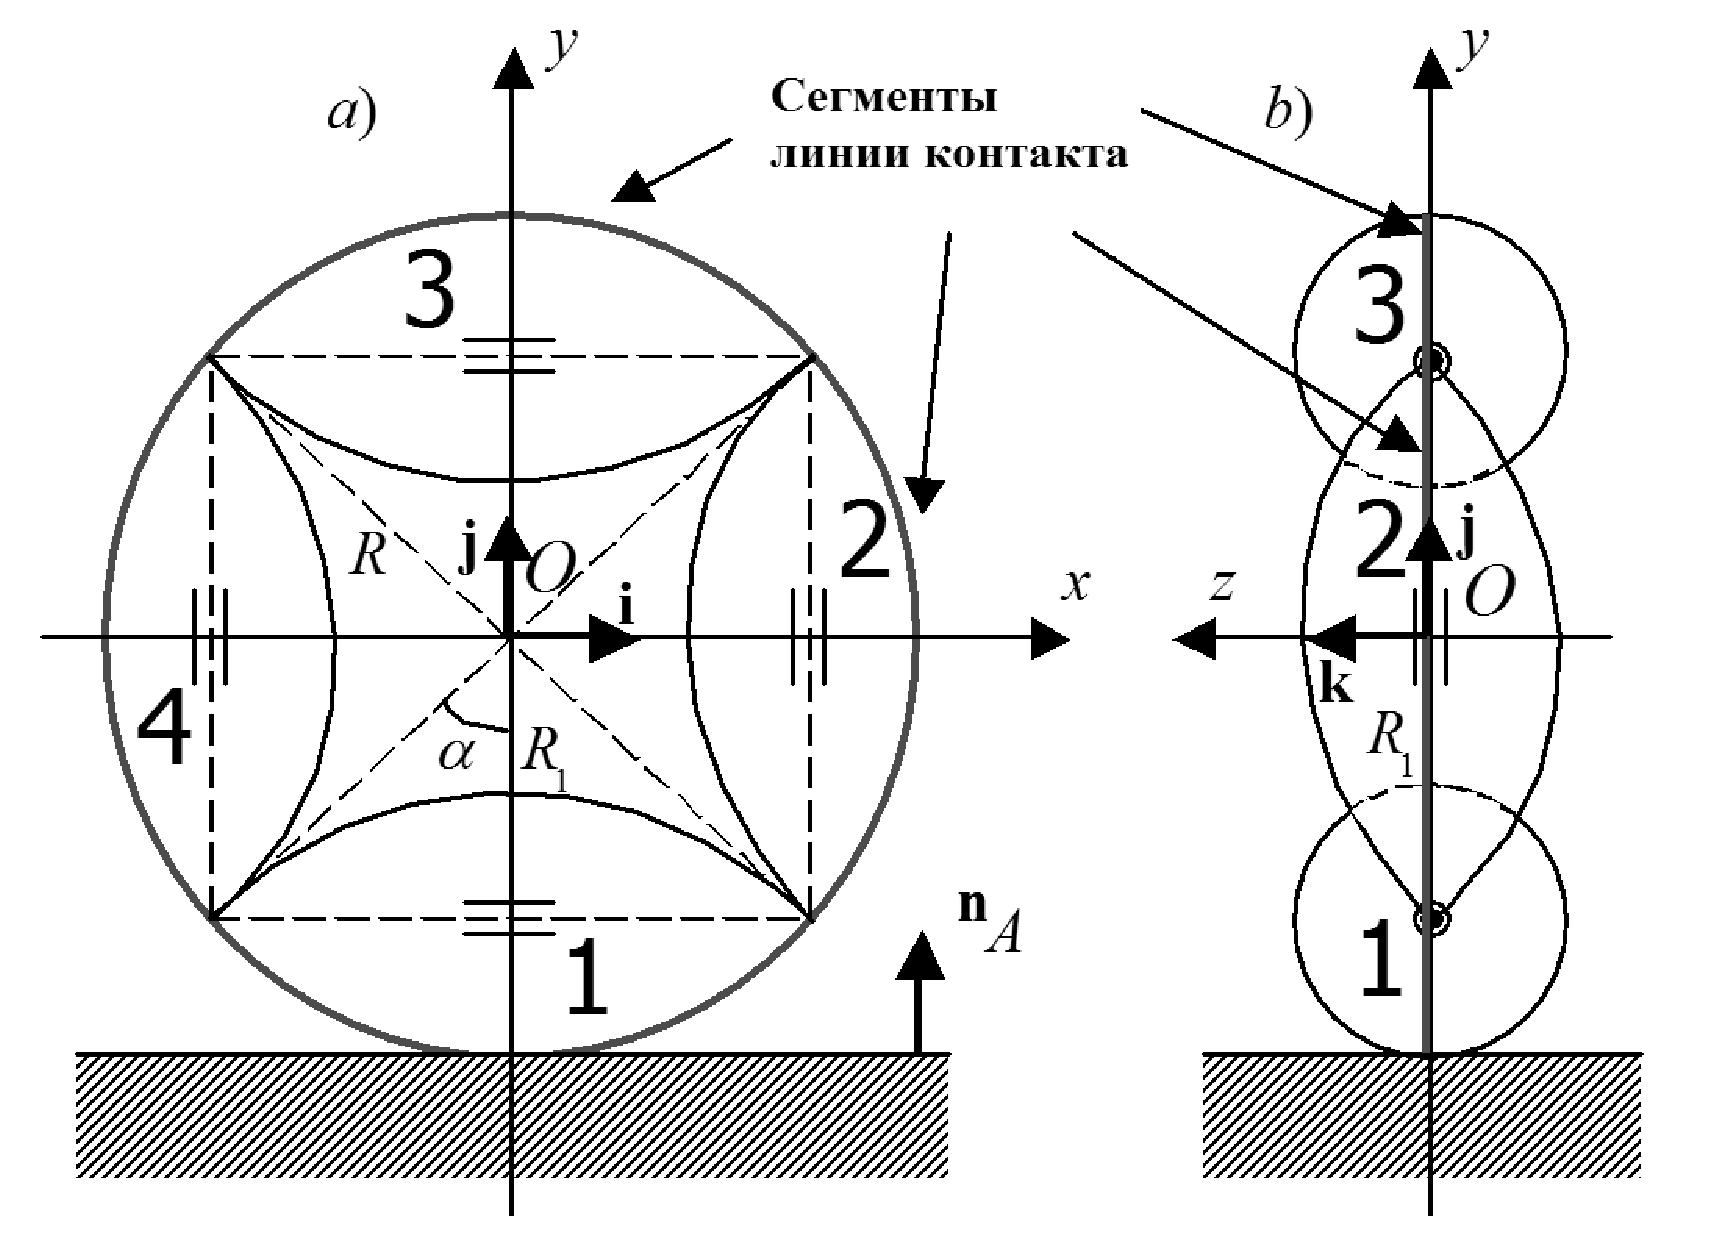
\includegraphics[width=13cm]{content/parts/3_friction/nd/OmniWheel.eps}
\caption{Омни-колесо в вертикальном положении: a) вид сбоку; b) вид спереди.}
\label{OmniWheel}
\end{figure}


%Так что в результате переключение контактов между роликами омни-колеса не приведет к нарушению регулярности движения в силу причин ударного характера. Заметим еще раз, что все описанное будет справедливо, если колесо все время остается в вертикальном положении.

% На следующем уровне сборки модели несколько колес соединяются с подвижной 
% платформой экипажа при помощи шарнирных связей. В нашем случае количество колес 
% может быть три или более (в зависимости от конструкции экипажа и модели 
% контактирования ролика с полом). На платформе они могут образовывать самые 
% разные конфигурации. В конкретном примере Рис.~\ref{Vehicle} имеется три 
% колеса, образующие равносторонний треугольник в горизонтальной плоскости $zx$. 
% Ось $y$ здесь предполагается вертикальной.

% \begin{figure}[htb]
% \centering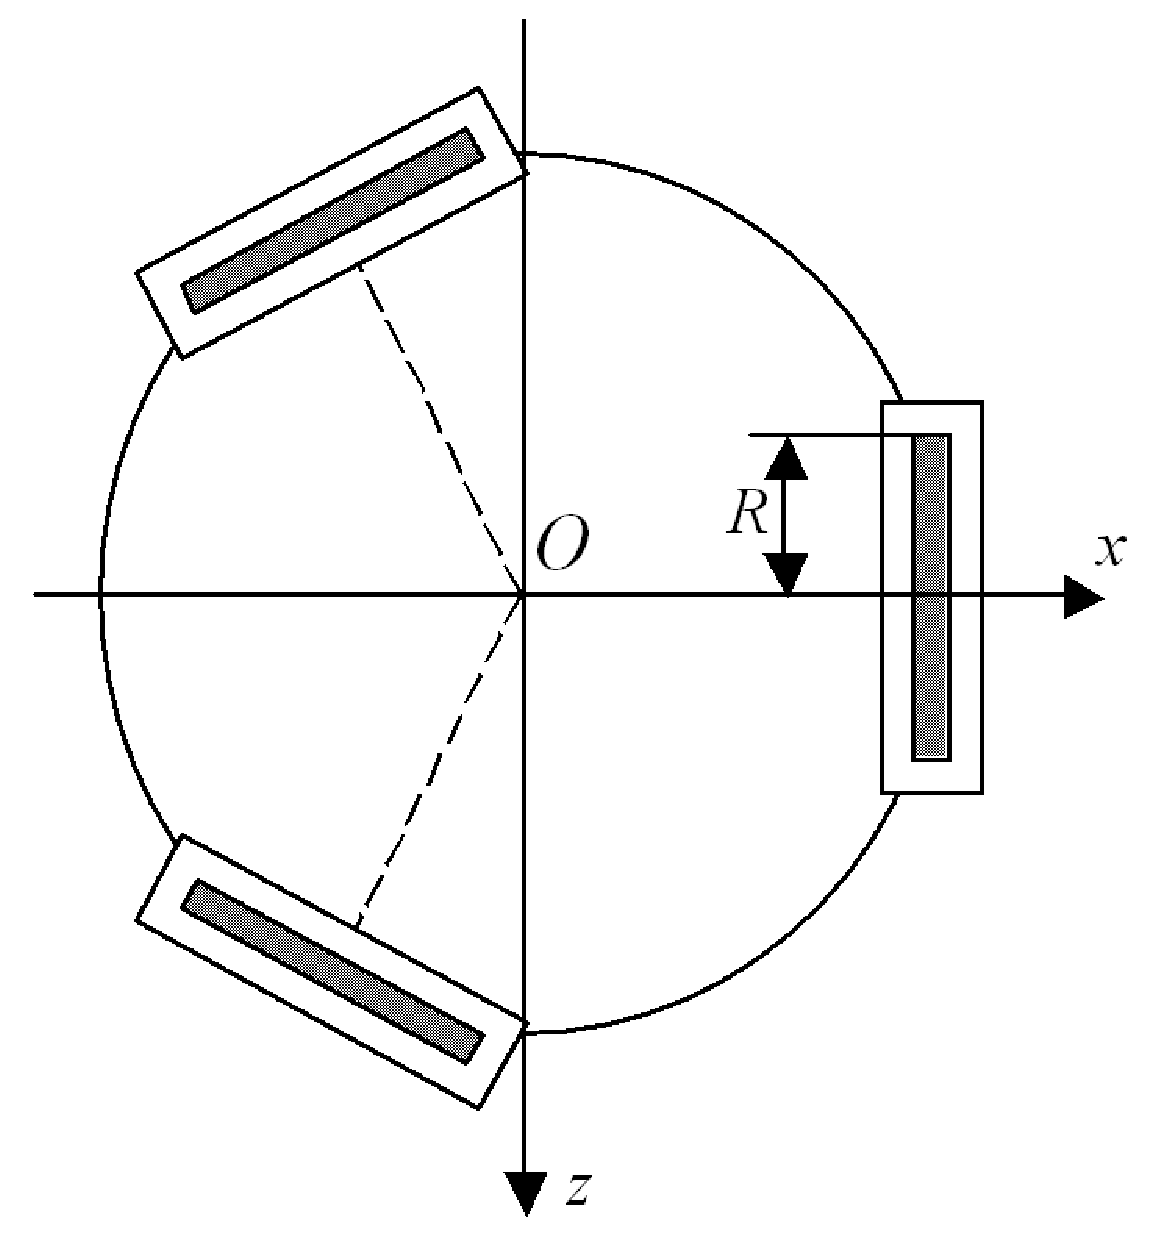
\includegraphics[width=9cm]{content/parts/3_friction/nd/Vehicle.eps}
% \caption{Трехколесный экипаж. Вид сверху.}
% \label{Vehicle}
% \end{figure}

% \section{Модель динамики отдельного ролика.\ }
\label{sec3}
Для начала составим формулы, задающие геометрическую одностороннюю связь контакта одного неусеченного ролика и плоскости. Введем оси $Oxyz$, жестко связанные с роликом, следующим образом: ...
Напомним, что ролик ограничен поверхностью вращения дуги окружности радиуса $l$ вокруг ее хорды, так что  уравнение поверхности имеет вид (см. фиг.~\ref{Roller}):
\begin{equation}
x^2+\left(\sqrt{y^2+z^2}+R_1\right)^2=R^2,
\label{3_1}
\end{equation}
ОБОЗНАЧЕНИЯ!!!
где $R$ --- радиус омни-колеса, $R_1=R\cos{\alpha }$ --- расстояние от центра
ролика до центра колеса, $\alpha =\pi /n$ --- половина центрального угла, под
которым ролик виден из центра колеса, $n$ --- количество роликов на колесе.

\begin{figure}[htb]
\centering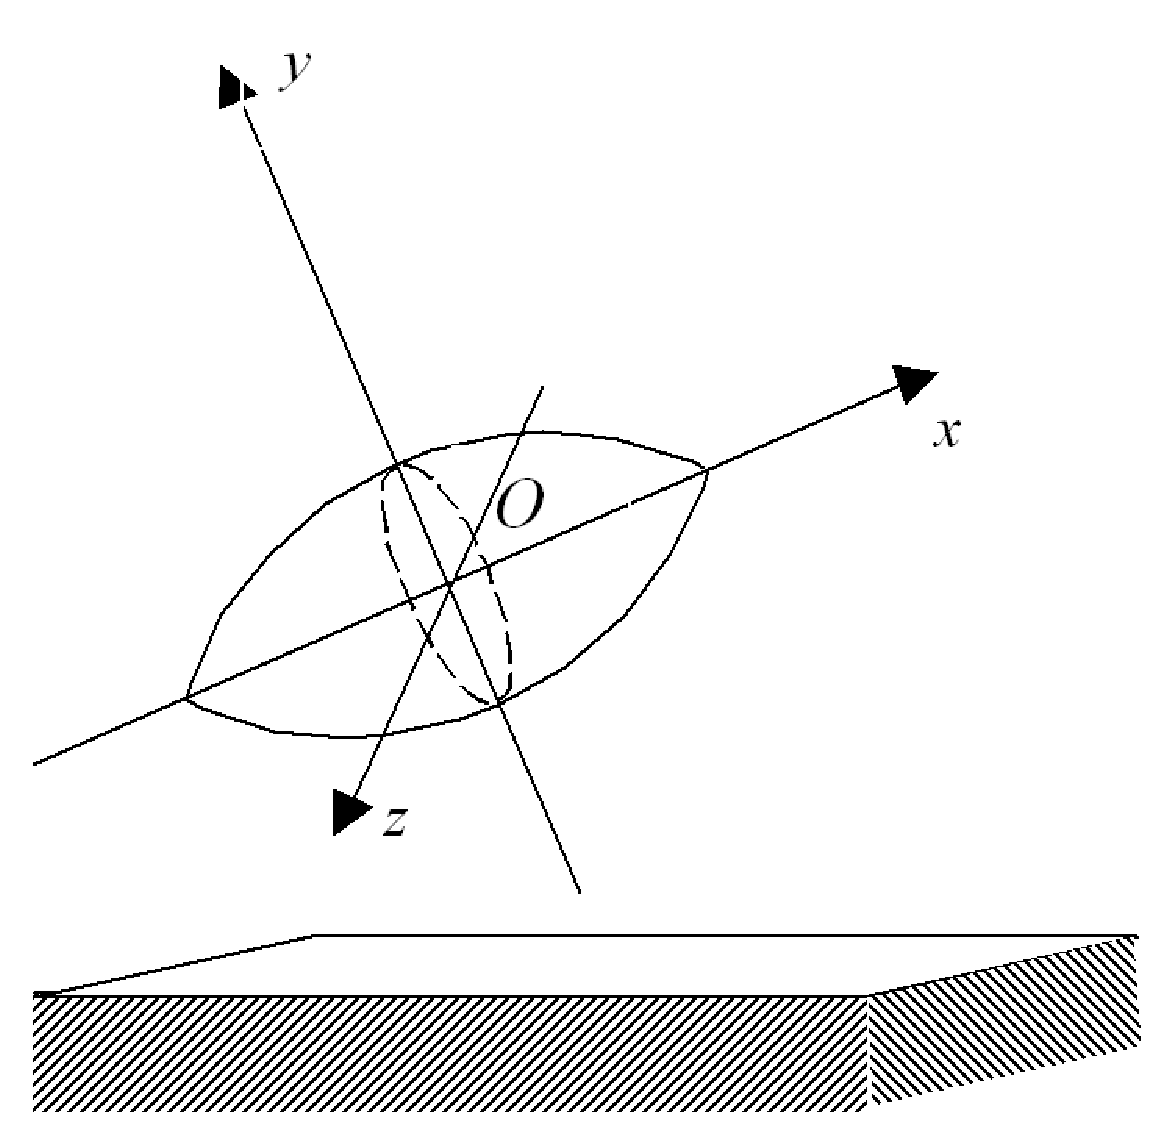
\includegraphics[width=10cm]{content/parts/3_friction/nd/Roller.eps}
\caption{Ролик над горизонтальной плоскостью. Вид сбоку.}
\label{Roller}
\end{figure}

\cite{Kosenko2007}\cite{Kosenko2006}

% Динамика поступательно-вращательного движения реализуется так, как это описано в, в виде уравнений Ньютона -- Эйлера. Причем для моделирования вращательного движения твердого тела используется алгебра кватернионов~\cite{KosenkoQuaternionRus,Kosenko1998}.

Сказать, что здесь можно острие!
И что мы этим воспользовались, но не только, а еще и усеченные тоже.
    МЫСЛЬ СКОЛЬЗИТЬ МОЖНО !.

Заметим, что эта поверхность имеет  в 
точках $x=\pm R\sin\alpha $ особенность, что в численных алгоритмах обычно приводит к аварийному завершению вычислительного процесса моделирования.

В нашей задаче положение спасает специфика конфигурации, обеспечивающей 
постоянство вертикального расположения омни-колес, так что касательная плоскость к поверхности ролика определена при любух значениях координат. При этом условии можно
указать явную формулу, позволяющую вычислить ближайшую к плоскости точку $P_B$
ролика (Рис.~\ref{ContactScheme}). Этой точке всегда <<противостоит>> её 
вертикальная проекция $P_A$ на плоскость (Рис.~\ref{ContactScheme}).

\begin{figure}[htb]
\centering\includegraphics[width=8cm]{content/parts/3_friction/nd/RollerSection_d_ib.png}
\caption{Схема отслеживания контакта: вид сбоку отдельного ролика.}
\label{ContactScheme}
\end{figure}

!!!!!!!!!!!!!!В последующем тексте:
меняем обозначения на принятые ранее, убираем произведение матриц.

Обозначим ${\bf i}$ --- орт оси ролика,
${\bf r}_B$ ---
радиус-вектор геометрического центра ролика в текущий момент времени и 
${\bf \gamma}$ --- орт нормали к плоскости,  в нашей задаче являющийся единичным вектором восходящей вертикали. 
%Плоскость условно обозначается нами телом с индексом $A$, ролик --- $B$. 
Введем орт ${\bf d}$ --- горизонтальный орт, перпендикулярный плоскости колеса
$$
{\bf d}=\dfrac{{\bf i}\times {\bf \gamma}}
              {\left| {\bf i}\times {\bf \gamma}\right|}.
$$
Пусть $O$ --- центр окружности, вращением дуги которой образована поверхность ролика(Рис.~\ref{ContactScheme}). (Заметим, что эта же точка является центром омни-колеса)  
Тогда, очевидно, отрезок $\overrightarrow{O_BO}$, расположенный в вертикальной
плоскости, будет иметь длину $R_1$ и задаваться формулой
$$
\overrightarrow{O_BO}=R_1{\bf d}\times {\bf i}_B.
$$
 Так что самая нижняя точка $P_B$ внешней 
поверхности ролика будет задаваться по формуле
\begin{equation}
{\bf r}_{P_B}={\bf r}_B+R_1{\bf d}\times T_B{\bf i}_B-R{\bf n}_A,
\label{3_2_0}
\end{equation}
поскольку точка $P_B$ лежит на упоминавшейся выше окружности на общей вертикали 
с точкой $O$. 

%Для вычисления положения точки $P_A$ нужно вторую координату 
%вектора ${\bf r}_{P_B}$ положить равной нулю
%\begin{equation}
%{\bf r}_{P_A}=\left( x_{P_B},0,z_{P_B}\right) ^T.
%\label{3_2_1}
%\end{equation}

Вся описанная выше вычислительная процедура будет справедлива только, если 
вектор $T_B{\bf i}_B$ имеет направление, ограниченное по вертикали углами
$\pm\alpha $. 
Если соответствующий угол превышает значение $\alpha$, то 
следует положить $P_B=B_{-}$, где $B_{-}$ --- левая концевая точка ролика. Если
же этот угол меньше величины $-\alpha $, нужно положить $P_B=B_{+}$, где 
$B_{+}$ --- правая концевая точка ролика.

В конечном итоге условие контактирования ролика и плоскости можно записать в 
виде
\begin{equation}
\left| T_B{\bf i}_B\cdot {\bf n}_A\right|\le\sin\alpha .
\label{3_2}
\end{equation}
Это условие, однако, позволяет из всего множества роликов колеса выделить 
нижний (контактирующий) и верхний. Чтобы отбросить случай последнего ролика
можно к последнему условию присоединить также требование 
\begin{equation}
y_B<R,
\label{3_3}
\end{equation}
где $y_B$ --- высота центра ролика относительно инерциальной системы координат.

Таким образом, конъюнкция условий (\ref{3_2}) и (\ref{3_3}) означает наличие
контакта. В противном случае, при отсутствии контакта, нормальная реакция 
отсутствует. С другой стороны, реализация контакта 
геометрически означает выполнение скалярного условия 
\begin{equation}
y_{P_B}=0,
\label{3_4}
\end{equation}
а его отсутствие --- также скалярного (альтернативного) условия
$$
F_n=0,
$$
где $F_n$ --- нормальная составляющая реакции (в данном случае отсутствующей) 
приложенной в точке $P_B$.

% \begin{figure}[htb]
% \centerline{
% 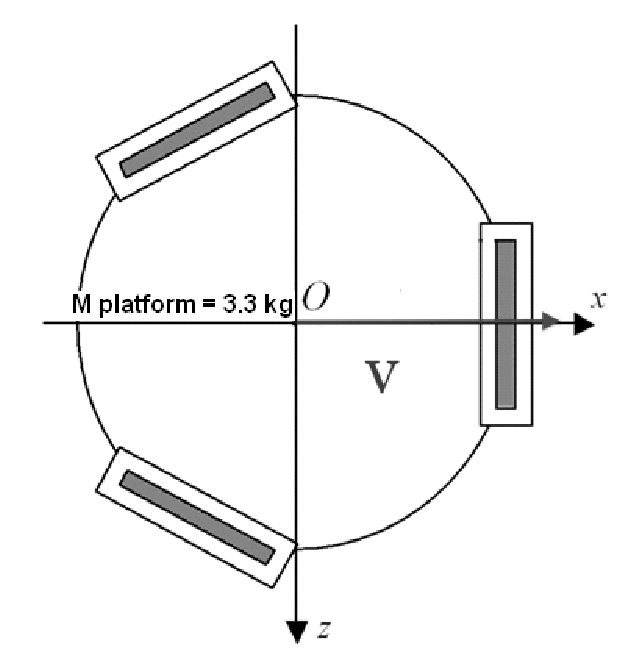
\includegraphics[width=7cm]{content/parts/3_friction/nd/Translat.eps}
% 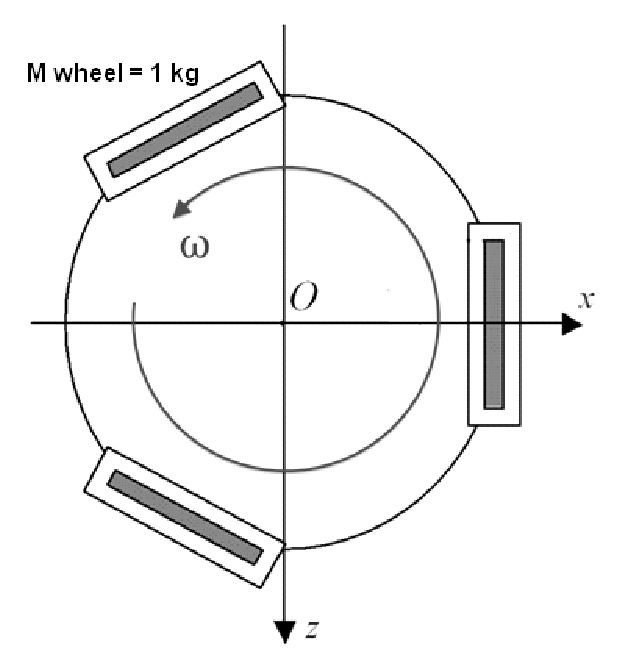
\includegraphics[width=7cm]{content/parts/3_friction/nd/Rotat.eps}
% }
% \caption{Типы движения при верификации модели.}
% \label{TypesOfMotion}
% \end{figure}

Вычислительная практика показала, что уравнения контакта в форме (\ref{3_4})
стабильно приводит к аварийному завершению процесса симуляции динамической 
модели ролика. Аналогичный результат получается, если в качестве уравнения 
контактирования использовать уравнение вида 
$$
v_n=0,
$$
где $v_n$ -- нормальная составляющая скорости точки контактирования, лежащей
на теле $B$, относительно тела $A$ (горизонтальной плоскости). И только 
уравнение вида
$$
\dot{v}_n=0
$$
приводит к требуемому результату -- корректной работе объекта контактирования
(реализованного в данном случае на языке Modelica~\cite{Fritzson}) в процессе 
симуляции модели. Вся реализация процесса контактирования 
выполнена в предположении точечного <<твердого>> контакта твердых тел без 
какой-либо податливости.

Колеса, собранные в экипаж, с неизбежностью будут сохранять вертикальное 
положение. Поэтому упрощенный алгоритм отслеживания контакта, описанный выше,
всегда будет работать правильно.

Поскольку ролики, вообще говоря, входят и выхоядят из состояния контакта с опорной плоскостью, то и силы трения и нормальные реакции приложены к роликам не во все время движения, и требуется указать кинематические условия, при которых имеется контакт.

Итак, ролик находится в контакте, если только если $\vec{s} \cdot \vec{e}_z < \cos\ddfrac{\pi}{n} $ и $ z_C < l $. В противном случае со стороны опорной плоскости к ролику не приложены силы. В случае контакта, сперва найдем координаты и скорость точки ролика, находящейся в данный момент на опорной плоскости:

$$ \vec{r}_C = \vec{r}_K + r\vec{s} - l\vec{e}_z + \lambda\vec{k}_1 $$
$$ \lambda = \ddfrac{\left(r\vec{s} - l\vec{e}_z\right)\cdot\vec{k}_2}{ \vec{k}_1\cdot\vec{k}_2} $$
$$ \vec{v}_C = \vec{v}_K + [ \vec{\omega}_{\text{рол}}, \overrightarrow{KC} ] $$

Тогда для определения реакций воспользуемся уравнениями:
$$ \vec{v}_C \cdot \vec{e}_z = 0 $$
$$ \vec{R}_{\text{к}} = \vec{F}_{\text{тр}} + N\vec{e}_z $$
Иначе $ \vec{R}_{\text{к}} = \vec{0} $

\section{Отслеживание контакта в случае \textit{mecanum} колеса}

Обозначим угол наклона оси ролика к плоскости колеса $\psi$. В предыдущей конфигурации этот угол равен нулю. Расширим алгоритм отслеживания контакта, описанный выше для случая $\psi = 0$ на конфигурацию \textit{mecanum}, $\psi > 0$. В этом случае, в первую очередь, отметим отличия в геометрической форме роликов. Каждый ролик -- это твердое тело, ограниченное поверхностью вращения некоторой кривой вокруг его оси. В случае $\psi = 0$ эта кривая -- дуга окружности, но при $\psi > 0$, для того, чтобы проекция внежней границы колеса на его плоскость оставалась окружностью, форма роликов должна быть более сложной \cite{Gfrerrer2008}.

\subsection{Неявный алгоритм отслеживания контакта}

Здесь, как и всюду, будем предполагать, что плоскость колеса вертикальна во все время движения.

Введем систему отсчета $O_A{\bf i}{\bf j}{\bf k}$, жестко связанную с колесом, с началом в его центре $O_A$. Вектор ${\bf k}$ направлен вдоль оси колеса, ${\bf i}$ и ${\bf j}$ лежат в его плоскости.

Введем также две вспомогательные системы отсчета $O_A{\bf i}_1{\bf j}_1{\bf k}_1$ и $O_B{\bf i}_2{\bf j}_2{\bf k}_2$, где $O_B$ -- центр ролика.

Вектор ${\bf i}_2$ направим вдоль оси симметрии ролика, см. фиг.~\ref{ContactScheme}.
Вектор ${\bf j}_2$ ортогонален ${\bf i}_2$ и лежит в вертикальной плоскости.
Третий вектор ${\bf k}_2$ определяется естественным образом как
$$
{\bf k}_2={\bf i}_2\times {\bf j}_2.
$$
% \begin{figure}[hb]
% \centerline{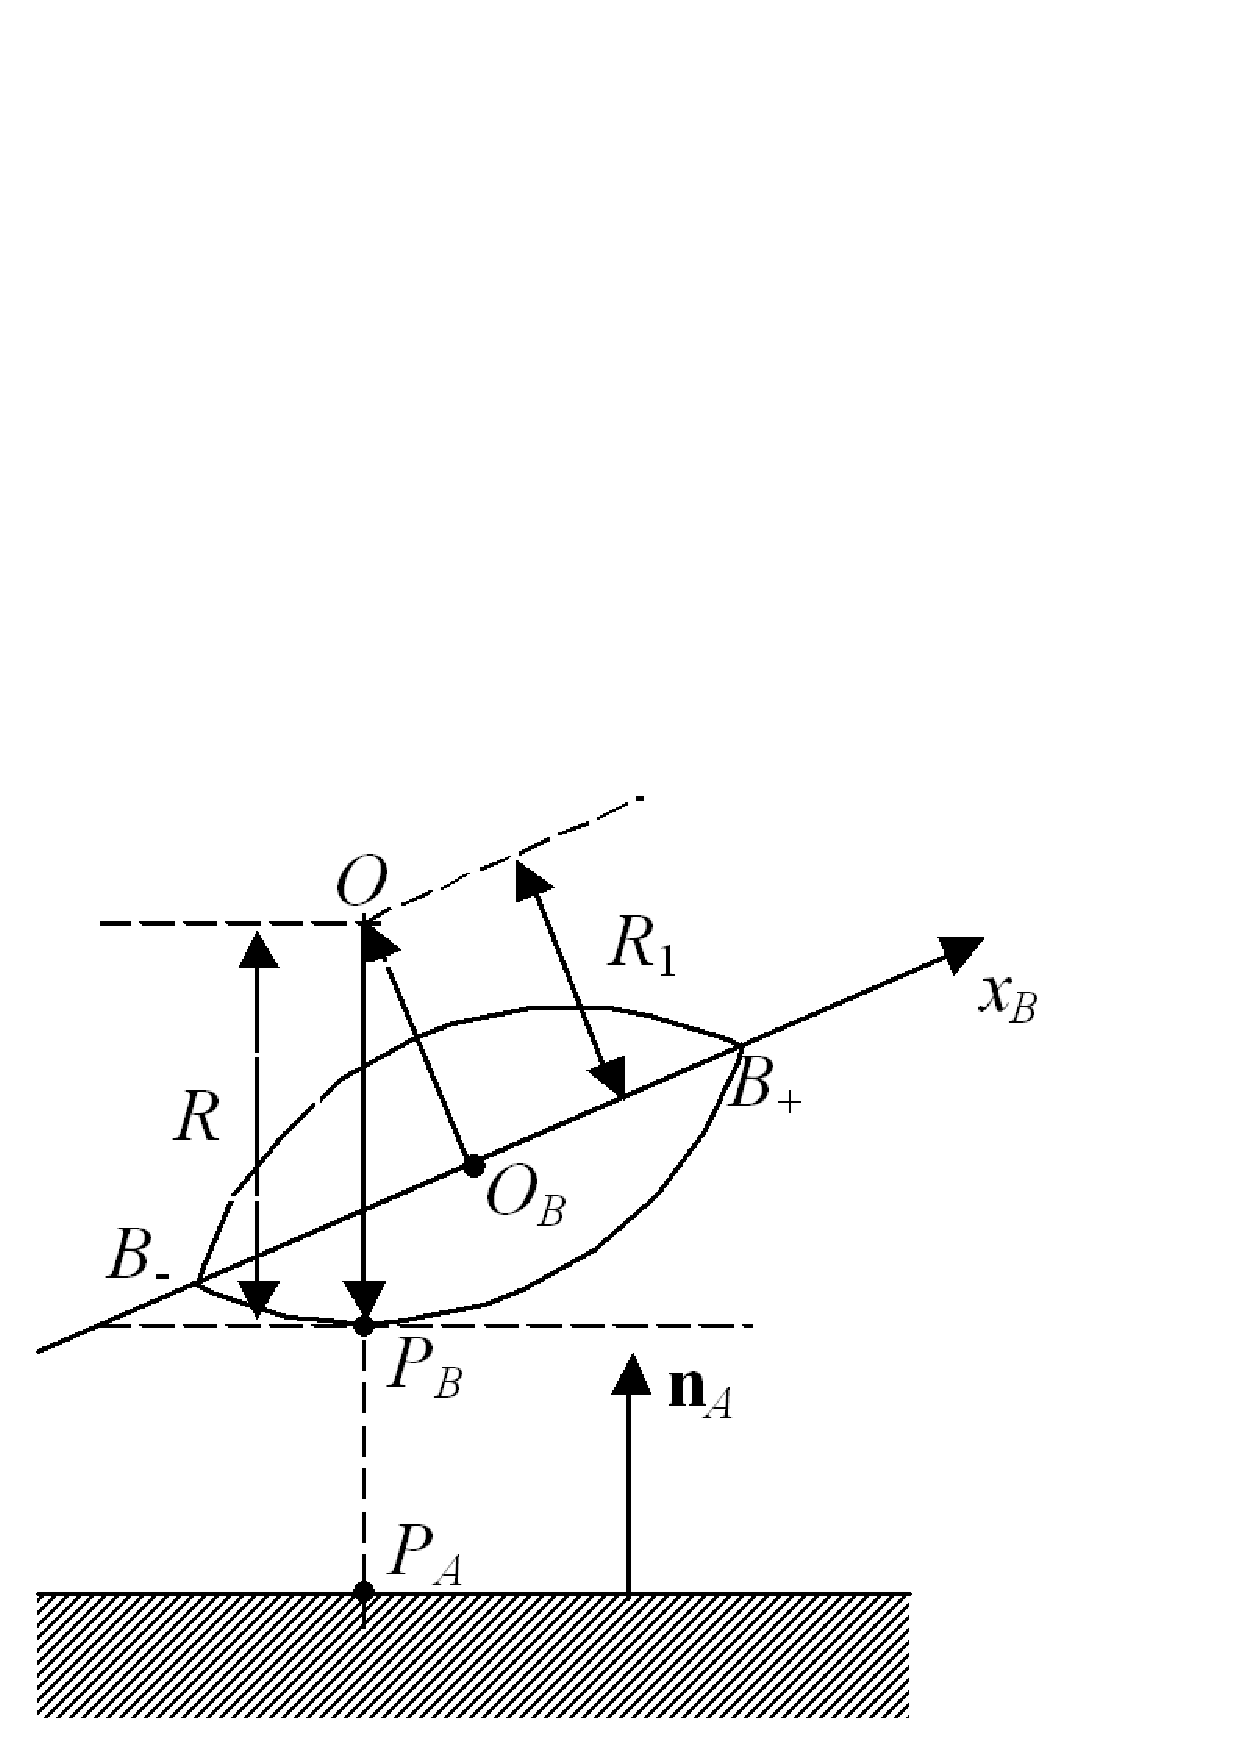
\includegraphics[bb= 0cm 0cm 20cm 17cm,scale=0.30]{RollerSection.png}}
% \caption{Contact tracking scheme.}
% \label{ContactScheme}
% \end{figure}

Во время счета компоненты всех векторов задаются относительно неподвижной системы отсчета, а положения и ориентации всех тел системы в момент времени $t\in [t_0,t_1]$ считаются известными.

Таким образом, для системы $O_B{\bf i}_2{\bf j}_2{\bf k}_2$, имеем:
$$
{\bf i}_2=T_B\cdot (1,0,0)^T,\quad\vecrho =
\left( {\bf r}_{O_A}-{\bf r}_{O_B}\right) /
\left| {\bf r}_{O_A}-{\bf r}_{O_B}\right| ,
$$
где $T_B$ -- матрица ориентации ролика, а единичный вектор $\vecrho$ направлен вдоль луча, выпущенного из центра колеса $O_A$ в сторону центра ролика $O_B$.

Вектор ${\bf i}_1$ лежит на пересечении плоскости колеса и горизонтальной плоскости.
${\bf k}_1 = {\bf k}$ ортогонален плоскости колеса и совпадает с одним из векторов базиса, связанного с колесом, и всегда горизонтален.
Тогда имеем ${\bf j}_1(t)=(0,1,0)^T$ и ${\bf i}_1(t)={\bf j}_1(t)\times {\bf k}_1(t)$.

Теперь рассмотрим соотношения, позволяющие вычислить компоненты базисных векторов векторов системы отсчета $O_B{\bf i}_2{\bf j}_2{\bf k}_2$.

Отметим, что вектор ${\bf i}_2$, направленный вдоль оси ролика, по определению не может принять вертикальное положение, если ролик находится в контакте с опорной плоскостью.
Более того, в случае \textit{mecanum} ролик повернут на постоянный угол $\psi > 0$ относительно оси $O_AO_B$, и потому во все время движения верно соотношение ${\bf i}_2\ne (0,1,0)^T$.
Таким образом, вектор ${\bf c}={\bf i}_2\times (0,1,0)^T$ также отличен от нуля.
Положим ${\bf k}_2={\bf c}/|{\bf c}|$. Теперь можно определить ${\bf j}_2$ как
${\bf j}_2={\bf k}_2\times {\bf i}_2$.

Для определения компонент вектора $\vecrho$ воспользуемся кинематическими соотношениями, условиями ортогональности векторов, следующими из определений введенных систем отсчета:
$$
\vecrho\cdot {\bf i}_2=0,\quad\vecrho\cdot {\bf k}_1=0.
$$
и их дифференциальными вариантами:
$$
\dfrac{d}{dt}\vecrho\cdot {\bf i}_2+\vecrho\cdot\dfrac{d}{dt}{\bf i}_2=0,\quad
\dfrac{d}{dt}\vecrho\cdot {\bf k}_1+\vecrho\cdot\dfrac{d}{dt}{\bf k}_1=0.
$$

Величина $c_{\beta }=\cos\beta ={\bf i}_2\cdot (0,1,0)^T$ косинуса угла $\beta $ наклона оси ролика к вертикали $(0,1,0)^T$ также играет важную роль в алгоритме отслеживания контакта.

Если текущее значение переменной величины $c_{\beta }$ меньше некоторого уровня $c_{\beta\max }$, и если одновременно расстояние от центра ролика $O_B$ до опорной плоскости меньше радиуса колеса $R$, то ролик находится в контакте с опорной плоскостью. В противном случае контакт отсутствует.

% Remark here that usually to arrange the unilateral constraint in the multibody
% system dynamics model the developer has to implement anything like hybrid 
% automata construct. In our omni wheel model on the contrary this is not the 
% case. It turned out sufficient to implement ``simple'' ``{\tt if}'' construct 
% to switch states ``contact'' and ``no contact'' for each individual roller, and
% simultaneously to advance forward ``contact'' state from one roller to its 
% neighbour. The whole picture looks like from time to time neighbouring rollers
% mutually exchange by their states.

На фиг.~\ref{ContactScheme} также легко видеть, что координаты точки $P_B$ контакта ролика и плоскости даются выражением
$$
{\bf r}_{P_B}={\bf r}_{O_B}+R_1\vecrho -R{\bf j}_1+\mu {\bf k}_1,
$$
где число $\mu$ требуется вычислить. Здесь величина $R_1$ равна расстоянию между точками $O_A$ и $O_B$.
Чтобы получить число $\mu$, умножим последнее уравнение скалярно на ${\bf k}_2$. Отсюда
$$
\mu =\left[R{\bf j}_1\cdot{\bf k}_2-R_1{\vecrho }\cdot {\bf k}_2\right] /
{\bf k}_1\cdot{\bf k}_2,
$$
поскольку ${\bf r}_{P_B}-{\bf r}_{O_B}$ лежит в вертикальном сечении осесимметричной поверхности ролика, и вектор ${\bf k}_2$ по построению ортогонален этому сечению. В результате радиус-вектор ${\bf r}_{P_B}$ точки контакта $P_B$ определяется однозначно.

\section{Явный алгоритм отслеживания контакта}

Еще одним способом вычисления компонент радиус-вектора ${\bf r}_{P_B}$ точки контакта point $P_B$ или, точнее, точки ролика, ближайшей к опорной плоскости, является применение следующего набора равенств.
Лучше всего этот способ иллюстрирует геометрическая схема на фиг.~\ref{fig:figure3}. Во-первых, имеем
$$
{\bf r}_{P_B}={\bf r}_{O_B}+\overrightarrow{CD}+\overrightarrow{DG},\quad
\overrightarrow{CD}=-m{\bf i}_2,\quad\overrightarrow{DG}=-h{\bf j}_1,
$$
где $m=R_1\sin q/\cos q/\cos\psi $, $h=R-R_1/\cos q$. Здесь $q$ -- текущее значение угла отклонения вектора ${\bf r}_{O_A}-{\bf r}_{O_B}$ от 
направления вектора $\overrightarrow{DO}$. Таким образом,
$$
\cos q=\vecrho\cdot{\bf n}_A,\quad\sin q=
\left({\bf n}_A\times\vecrho\right)\cdot {\bf k}_1.
$$
\begin{figure*}[ht]
\centerline{\includegraphics[scale=0.7]{content/parts/3_friction/mo2015/stepanov.png}}
\caption{Явная схема отслеживания контакта}
\label{fig:figure3}
\end{figure*}

Поясним фиг.~\ref{fig:figure3} более детально.
В части (а) приведена проекция колеса на его плоскость и соответственно, проекция ролика, находящегося в общем положении так, что его ось находится под углом к плоскости проекции.
Далее, $G$ -- точка контакта между роликом и опорной горизонтальной плоскостью в настоящий момент, $m'$ -- отрезок $DC$ проекции оси ролика на плоскость колеса. Лекго видеть, что длина этой проекции равна $m'=m\cos\psi$, поскольку ось ролика $AB$ повернута вокруг прямой $OC$ на угол $\psi$, см. вертикальное сечение, содержащее ось ролика в части (b).
Таким образом, чтобу получить точку контакта $P_B$ ($G$ на рис.), нужно пройти два отрезка прямых от центра ролика $O_B$ ($C$ на рис.): (a)~отрезок $CD$ оси ролика длины $m$; 
(b)~отрезок $DG$ вертикали длины $h$.
Как было отмечено выше, все величины требуется явно выразить через известные координаты.

Чтобы исключить <<перекрытие>> роликов, т.е. ситуацию, при которой два ролика могут находиться в контакте одновременно, более чем при одном (граничном) значении угла поворота колеса, необходимо ограничить длины роликов величиной (см. фиг.~\ref{fig:figure3})
$$
L=2R\sin\alpha / \cos\psi,
$$
и при этом их концы оказываются усечены. Подробно форма кривой, образующей поверхность роликов, описана в \cite{Gfrerrer2008}.
При такой конструкции переход колеса с одного ролика на другой происходит мгновенно.
Отметим, что при этом след колеса на плоскости имеет разрыв, поскольку точка контакта мгновенно переходит на противоположный <<борт>> колеса. Это обстоятельство, впрочем, не препятствует эффективному численному решению.

Описанные алгоритмы отслеживания контакта дают практически одинаковые результаты, относительные различия между которыми имеют порядок $10^{-8}$. Предсказуемо, явный алгоритм быстрее приблизительно в $1.5$ раза.

\section{Моделирование трения в контакте}

Вычислительная практика показала, что уравнения контакта в форме (\ref{3_4})
стабильно приводит к аварийному завершению процесса симуляции динамической 
модели ролика. Аналогичный результат получается, если в качестве уравнения 
контактирования использовать уравнение вида 
$$
v_n=0,
$$
где $v_n$ -- нормальная составляющая скорости точки контактирования, лежащей
на теле $B$, относительно тела $A$ (горизонтальной плоскости). И только 
уравнение вида
$$
\dot{v}_n=0
$$
приводит к требуемому результату -- корректной работе объекта контактирования
(реализованного в данном случае на языке Modelica~\cite{Fritzson}) в процессе 
симуляции модели. Заметим, что вся реализация процесса контактирования 
выполнена в предположении точечного <<твердого>> контакта твердых тел без 
какой-либо податливости.

Для каждого ролика модели омни-экипажа при контактировании <<включается>>
используемая здесь модель трения. Это <<простейший>> закон Амонтона -- Кулона
сухого трения. На самом деле вместо этого нами используется кусочно-линейная 
аппроксимация точного закона трения~\cite{Kosenko2006unilat}. Эта аппроксимация 
обеспечивает высокую точность вычисления движения тел на больших интервалах 
времени~\cite{Novozhilov1991}. Заметим, что и в общем случае реализация модели 
неудерживающей связи основывается на результатах, обозначенных в 
работе~\cite{Kosenko2006unilat}.

Конструкция омни-колеса такова, что в каждый данный 
момент времени имеется имеется только один контакт. Остальные ролики <<висят>>
над полом. При этом механическая связь между полом и, <<висящим>> на ободе
колеса, роликом не исчезает -- алгоритм отслеживания контакта продолжает 
работать, генерируя в качестве реакций нулевые усилия и моменты.

В случае фактического выполнения контакта помимо нормальной реакции вычисляется
также её касательная составляющая, симулирующая силу трения. Для касательного 
контактного усилия имеется (как и для нормального) множество различных моделей. 
Мы остановились на реализации простейшего случая -- модели сухого трения при 
одноточечном твердотельном контакте. При этом, как известно~\cite{Novozhilov1991}, 
идеальный <<сухой>> случай реализовать не удается. Вместо разрывной функции 
sign от касательной скорости относительного скольжения контактирующих 
поверхностей используется её регуляризованный в нуле вариант. В нашем случае 
вместо функции знака sign применяется функция линейного насыщения, имеющая в 
окрестности нуля <<крутой>> линейный участок. Для таких функций известен 
результат~\cite{Novozhilov1991} о близости аппроксимирующего движения и движения, соответствующего <<точному>> случаю разрывной функции sign.

В процессе отладки модели рассматривались автономные движения отдельного 
омни-колеса.

Заметим, что перед началом процесса редукции индекса системы 
дифференциально-алгебраических уравнений полной модели экипажа, реализованного
в программном обеспечении лаборатории динамического моделирования 
Dymola~\cite{Dymola}, эта модель составляется из: а) твердого тела платформы
омни--экипажа; б) трех твердых тел -- моделей омни--колес; в) двенадцати 
твердых тел роликов, размещенных на колесах. В соответствии, например, 
с~\cite{Kosenko2007} для каждого объекта, моделирующего твердое тело, 
реализуются шесть обыкновенных дифференциальных уравнений (ОДУ) Ньютона для
движения центра масс тела плюс семь ОДУ Эйлера для вращательного движения тела
вокруг центра масс. В последнем случае имеется четыре кинематических уравнения
Эйлера для кватерниона ориентации тела плюс три динамических уравнения Эйлера
для вектора угловой скорости твердого тела. В результате полная модель экипажа
задается системой ОДУ порядка $16\cdot 13=208$. Кроме этого, объекты 
механических связей могут генерировать дополнительные дифференциальные 
уравнения.

\begin{figure}[htb]
\centerline{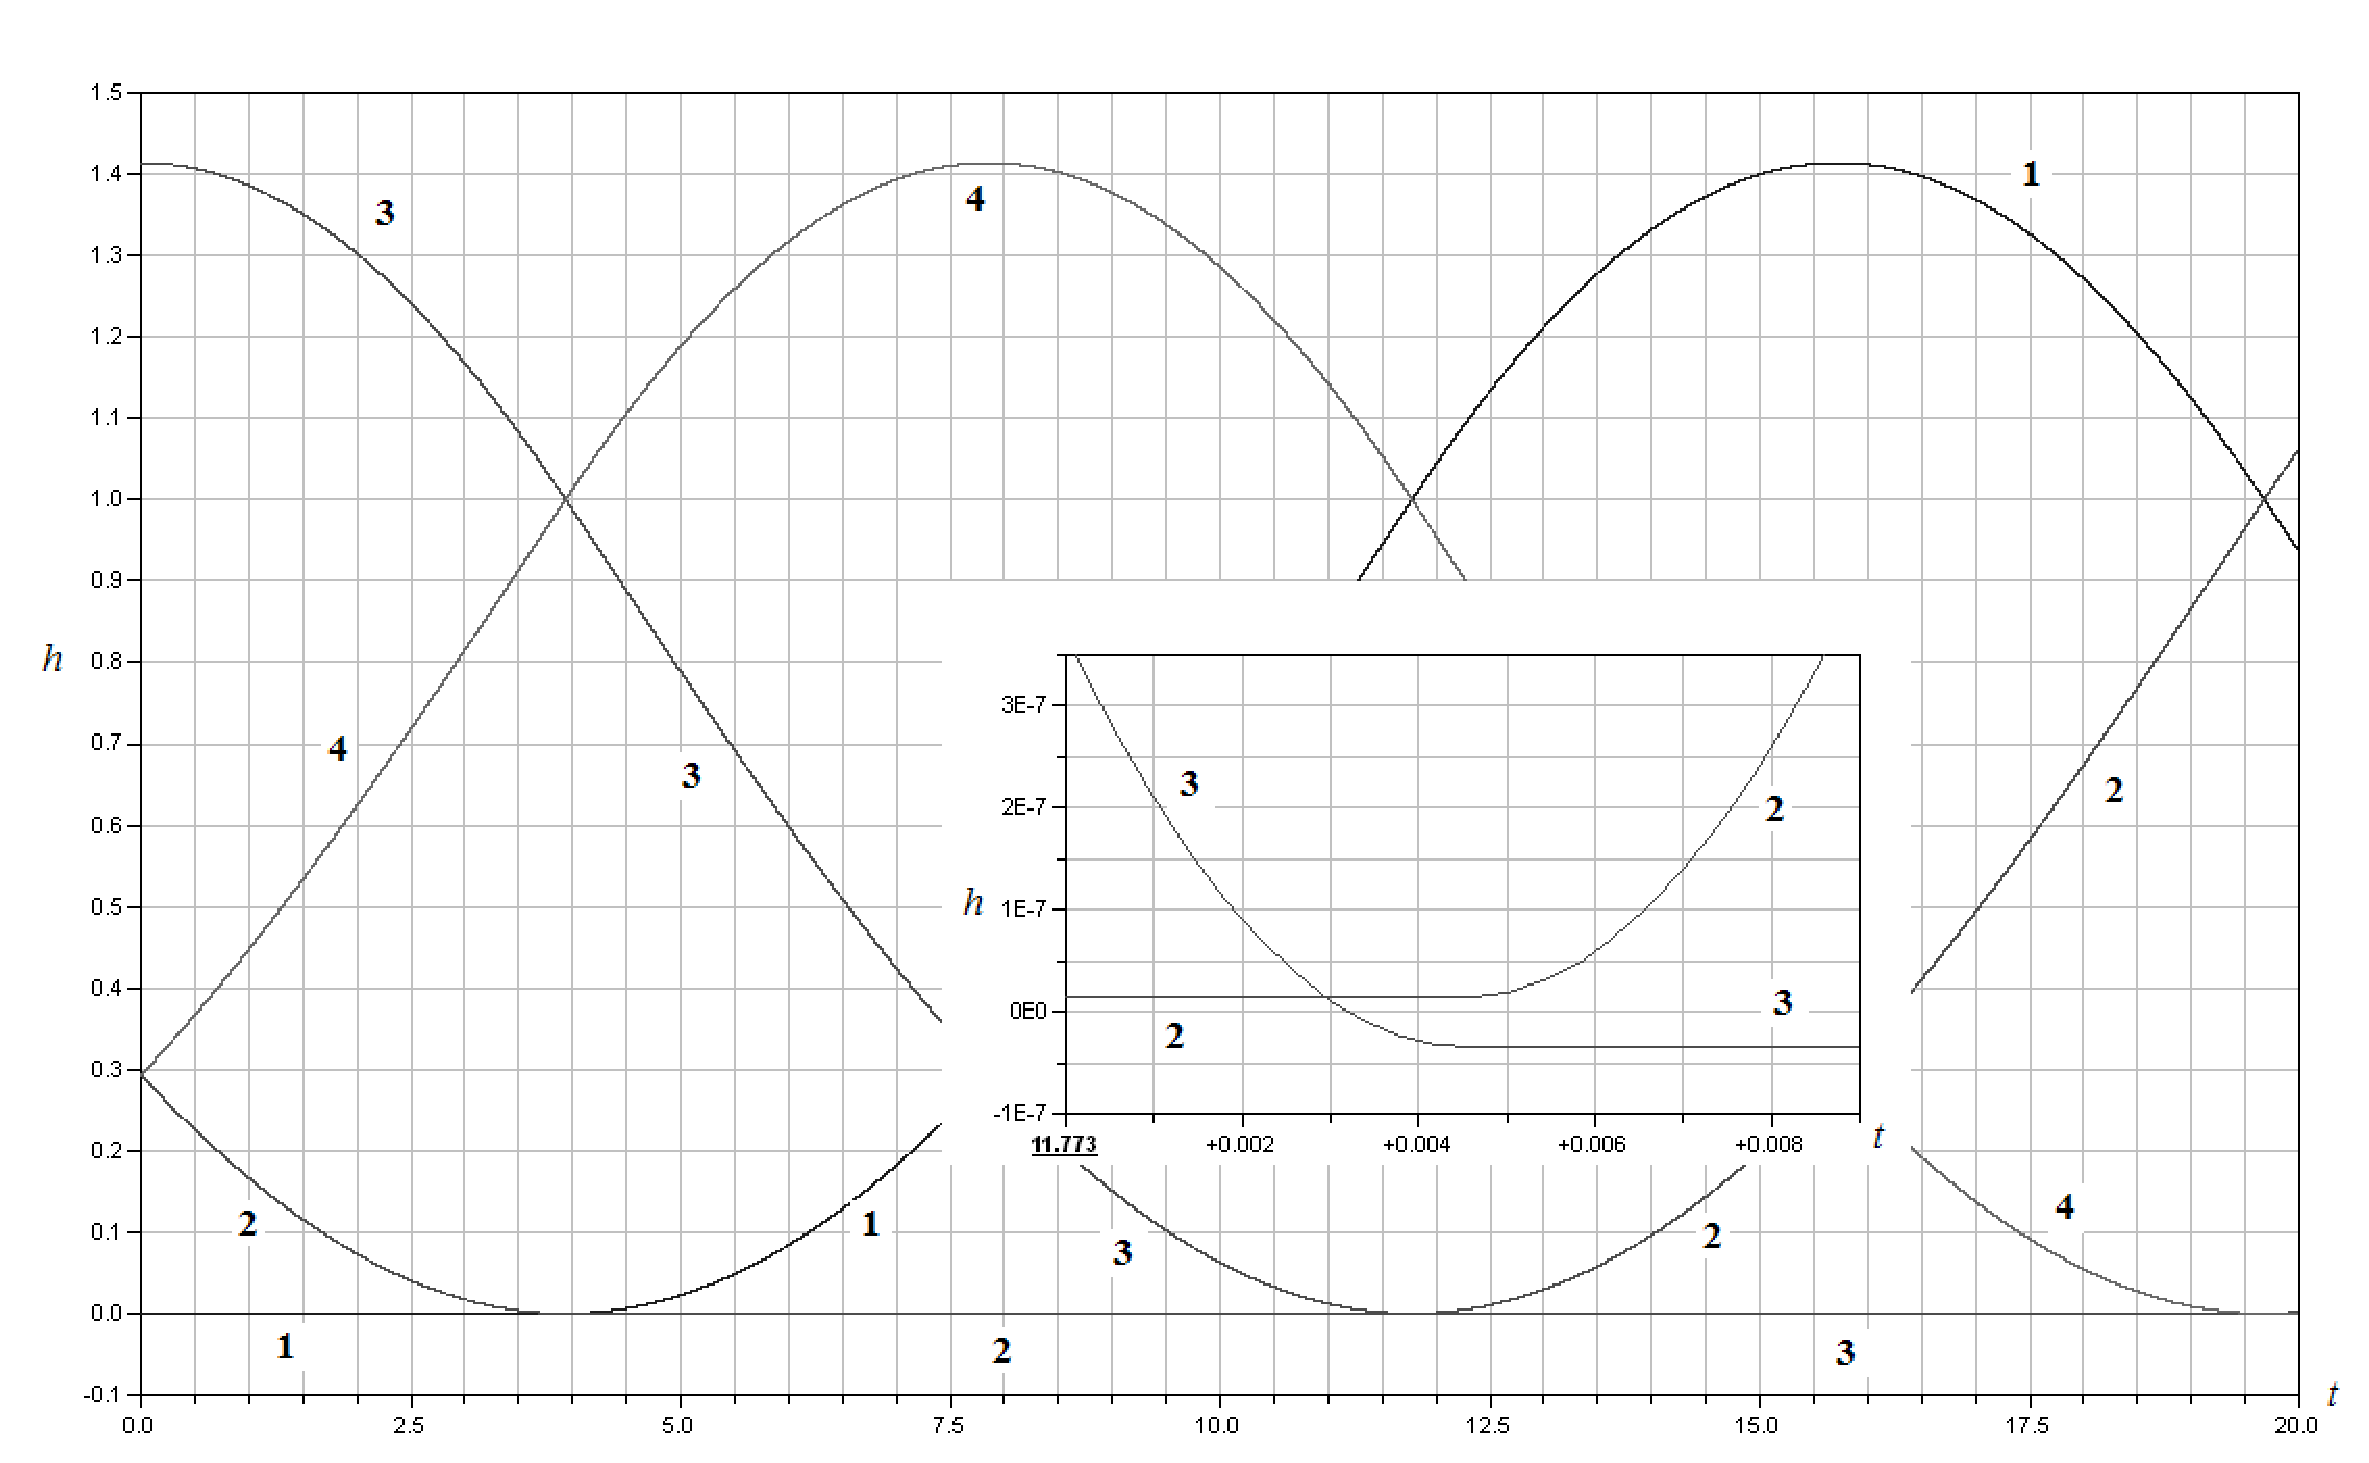
\includegraphics[width=15cm]{content/parts/3_friction/nd/Figure11.eps}}
\caption{Процесс замещения роликов в контакте.}
\label{fig1}
\end{figure}

Эволюция процесса контактирования для отдельного катящегося омни-колеса 
показана на Рис.~\ref{fig1}, где представлены зависимости функций расстояний 
$h$ (фактически -- высот) между горизонтальной плоскостью (полом) и роликами 
одного и того же колеса, находящимися в разных фазах (перед контактом, в 
контакте, после контакта). Функция высоты отдельного ролика помечена номером 
этого ролика. В увеличенном масштабе показан момент безударного гладкого 
переключения поверхностей контактирования роликов и горизонтальной плоскости.

Одновременно можно наблюдать точность соблюдения неудерживающей связи 
(Рис.~\ref{fig2}). Здесь обнаруживается процесс постепенного <<расползания>>
вычислительной ошибки -- расстояние между контактирующими телами медленно, для
каждого последующего ролика в контакте, увеличивается. В то же время, 
абсолютная величина ошибки остается пренебрежимо малой -- около $10^{-7}$
от единицы длины.

\begin{figure}[htb]
\centerline{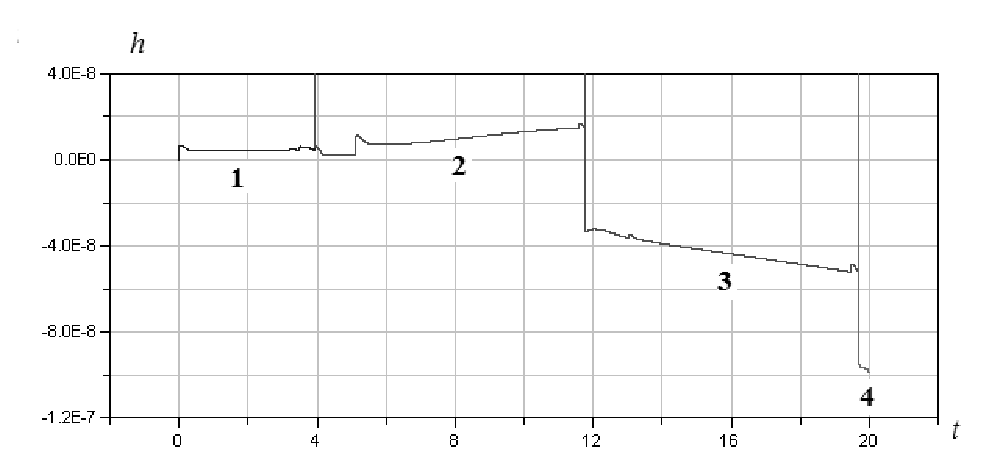
\includegraphics[width=15cm]{content/parts/3_friction/nd/Figure21.eps}}
\caption{Точность сохранения неудерживающей связи.}
\label{fig2}
\end{figure}

\section{Результаты численного моделирования}

В настоящем разделе описаны результаты двух видов расчетов. Во-первых, проведенной верификации модели экипажа на плоскости с регуляризованным сухим трением в сравнении с безынерционной моделью. Сравнение устроено при стремлении доли массы ролика в общей массе омни-колеса к нулю. Во-вторых, качественно сравнивается движение экипажа на плоскости с вязким трением с достаточно большим коэффициентом и движение модели, построенной в главах 1 и 2.

\subsection{Верификация модели с сухим трением}

Для проверки взаимной корректности безынерционной модели и модели с сухим трением проведены численные испытания, в которых, при прочих равных, изменялась величина $\massrel$ -- отношение массы одного ролика к массе колеса в целом. В этом случае оказалось, что при уменьшении данного параметра движение экипажа и омни-колес неограниченно приближаются к соответствующим функциям решения задачи Коши, получаемым в силу дифференциальных уравнений движения, используемых в работе~\cite{Borisov2011}, в которых динамика роликов не учитывается. При этом остальные параметры экипажа, такие как массы его частей, их моменты инерции, геометрические размеры, положения, а также начальные данные -- скорость центра масс и угловая скорость платформы, задавались согласованными между двумя моделями. Как и в главах 1 и 2, рассматривается симметричная конфигурация экипажа. Однако концы роликов в данном рассмотрении не усекаются: в силу выбора модели контактных сил и построенного явного алгоритма отслеживания контакта, особенность на острии ролика не препятствует проведению расчетов. Количество роликов $n$ равно $4$. Рассмотрены два типа начальных условий $\vec{v}(0) = (v_0, 0, 0)^T, \omega(0) = \omega_0$ (см. рис.~\ref{fig:my_exp_setup}):
\begin{enumerate}
\item экипаж имеет начальную линейную скорость в направлении одного из колес и не закручен (ожидаемый результат - центр масс экипажа движется вдоль оси $Ox$, экипаж не вращается),
\item экипаж закручен вокруг вертикальной оси, проходящей через его центр масс, скорость центра масс равна нулю (ожидаемый результат - экипаж вращается вокруг своей вертикальной оси симметрии, и центр масс покоится).
\end{enumerate}
Значения отношения $\massrel$ массы ролика к общей массе колеса принимали в обоих случаях значения от $10^{-6}$ до $10^{-1}$ с шагом $1$ по порядку малости.

\begin{figure}[!ht]
    \centering
    \includegraphics[width=0.95\textwidth]{content/parts/3_friction/diploma/img/art/my_exp_setup.png}
    \caption{Параметры экспериментов}
    \label{fig:my_exp_setup}
\end{figure}

В таблице\upr{tab:verif} приведены величины отличий угла курса $\theta$ экипажа и координат центра масс $x, y$ к моменту безразмерного времени $t = 10$. Отличия уменьшаются с уменьшением порядка величины отношения массы одного ролика $m_{\text{рол}}$ к суммарной массе колеса $m_{\text{к}}$.

\begin{table}[]\label{tab:verif}
    \begin{tabular}{l|l|l}
     & Движение $1$ & Движение $2$ \\ \hline
    $\frac{m_{\text{рол}}}{m_{\text{к}}}$ &
    $\Delta \theta$ &
    $\max(|\Delta x|, |\Delta y|)$ \\ \hline
    $10^{-1}$ & $\approx 1$       & $\approx 1$       \\
    $10^{-2}$ & $\approx 10^{-1}$ & $\approx 0.5$     \\
    $10^{-3}$ & $\approx 10^{-2}$ & $\approx 10^{-1}$ \\
    $10^{-4}$ & $\approx 10^{-3}$ & $\approx 10^{-2}$ \\
    $10^{-5}$ & $\approx 10^{-3}$ &                   \\
    $10^{-6}$ & $\approx 10^{-4}$ & 
    \end{tabular}
    \caption{Порядок различий в значениях угла курса платформы $\theta$ и координат центра масс $x, y$ экипажа при движениях $1$ и $2$ и уменьшении $\massrel$}
\end{table}

На рис.~\ref{fig:exp_examples} приведены примеры траектории центра масс $y(x)$ и зависимости $\psi(t)$ угла поворота $\psi$ платформы вокруг вертикальной оси, проходящей через её центр, для случаев 1) и 2). Кривые $y(x)$, изображающие траектории центра масс, соответствуют, в сущности, точке -- началу координат -- в случае $v_0 = 0, \omega_0 = 1$, и отрезку прямой, совпадающей с осью $x$, в случае $v_0 = 1, \omega_0 = 0$, т.к. масштаб отображения таков, чтобы были видны отклонения от точных значений, возникающие в силу вычислительной погрешности, но сами эти отклонения имеют порядок малости, позволяющий считать их нулевыми. Аналогичное утверждение верно и для зависимости угла поворота платформы $\psi$ от времени в случае поступательного движения - полученная зависимость близка к постоянной.

Ниже представлены результаты нескольких численных экспериментов. Во всех случаях величины, изображенные на рис.~\ref{fig:exp_examples}, демонстрируют поведение, не различимое в масштабе рис.~\ref{fig:exp_examples}, и поэтому приведены лишь расхождения между построенной нами моделью и верификационной идеализацией, которые и представляют интерес. Также представлена абсолютная величина скорости скольжения в точке контакта в физической модели.

Графики зависимости скорости скольжения от времени показывают, что скольжение имеет место в окрестности момента смены роликов. Для вращательного движения это объясняется наличием того же динамического эффекта раскручивания роликов, что был обнаружен в главах 1 и 2: скользят именно вновь входящие в контакт ролики, но не ролики, уже находящиеся в контакте достаточное время. В случае поступательного движения платформы экипажа дополнительно возникает раскручивание роликов задних колес, находящихся в контакте, поскольку для идеального качения при подходе к острию, ролику необходима бесконечная угловая скорость собственного вращения, т.к. его радиус вблизи острия стремится к нулю.

Видно, что с ростом доли массы роликов в общей массе колеса скольжение в контакте становится существеннее, изменяясь от пренебрежимо малого при $\massrel = 10^{-6}$ до весьма существенного уже при $\massrel = 10^{-3}$. Тем не менее, расхождения траектории и угла поворота платформы малы, а скольжение наблюдается лишь в точках колеса, которые в промышленных конструкциях не присутствуют (см. Обзор), что и позволяет считать верификацию проведенной.
\newpage

% EXAMPLES
\begin{figure}[h]
\centering
\begin{subfigure}{.47\textwidth}
    \centering
    \includegraphics[width=\textwidth]{content/parts/3_friction/diploma/img/res/example_v_0_0_omega_1_frac_1e-1_n_4_time_10s.png}
    \caption{$\massrel = 0,1, v_0 = 0, \omega_0 = 1$}
    \label{fig:exp_example_omega}
\end{subfigure}%
\hspace{5pt}
\begin{subfigure}{.47\textwidth}
    \centering
    \includegraphics[width=\textwidth]{content/parts/3_friction/diploma/img/res/example_v_1_0_omega_0_frac_1e-1_n_4_time_10s.png}
    \caption{$\massrel = 0,1, v_0 = 1, \omega_0 = 0$}
    \label{fig:exp_example_v}
\end{subfigure}
\caption{Примеры траекторий, характера изменения угла и смены номеров роликов в контакте для двух типов начальных условий. На нижнем графике - номер ролика в контакте, см. рис.~\ref{OmniWheel}}
\label{fig:exp_examples}
\end{figure}
\newpage

\begin{figure}[h]
\begin{center}\begin{equation*}\begin{array}{cc}
\includegraphics[width=7cm, viewport=0 0 395 745,clip]{content/parts/3_friction/diploma/img/res/comparison_v_0_0_omega_1_frac_1e-1_n_4_time_10s.png} & \includegraphics[width=7cm, viewport=0 0 395 745,clip]{content/parts/3_friction/diploma/img/res/comparison_v_0_0_omega_1_frac_1e-2_n_4_time_10s.png}\\
\massrel = 10^{-1}, v_0 = 0, \omega_0 = 1 & \massrel = 10^{-2}, v_0 = 0, \omega_0 = 1\\
\end{array}\end{equation*}\end{center}
\caption{Движение 1 экипажа на плоскости с сухим трением, $\massrel = 10^{-1}, 10^{-2}$}
\end{figure}
\newpage

\begin{figure}[h]
\begin{center}\begin{equation*}\begin{array}{cc}
\includegraphics[width=7cm, viewport=0 0 395 745,clip]{content/parts/3_friction/diploma/img/res/comparison_v_0_0_omega_1_frac_1e-3_n_4_time_10s.png} & \includegraphics[width=7cm, viewport=0 0 395 745,clip]{content/parts/3_friction/diploma/img/res/comparison_v_0_0_omega_1_frac_1e-4_n_4_time_10s.png}\\
\massrel = 10^{-3}, v_0 = 0, \omega_0 = 1 & \massrel = 10^{-4}, v_0 = 0, \omega_0 = 1\\
\end{array}\end{equation*}\end{center}
\caption{Движение 1 экипажа на плоскости с сухим трением, $\massrel = 10^{-3}, 10^{-4}$}
\end{figure}
\newpage

\begin{figure}[h]
\begin{center}\begin{equation*}\begin{array}{cc}
\includegraphics[width=7cm, viewport=0 0 395 745,clip]{content/parts/3_friction/diploma/img/res/comparison_v_0_0_omega_1_frac_1e-5_n_4_time_10s.png} & \includegraphics[width=7cm, viewport=0 0 395 745,clip]{content/parts/3_friction/diploma/img/res/comparison_v_0_0_omega_1_frac_1e-6_n_4_time_10s.png}\\
\massrel = 10^{-5}, v_0 = 0, \omega_0 = 1 & \massrel = 10^{-6}, v_0 = 0, \omega_0 = 1\\
\end{array}\end{equation*}\end{center}
\caption{Движение 1 экипажа на плоскости с сухим трением, $\massrel = 10^{-5}, 10^{-6}$}
\end{figure}
\newpage

\begin{figure}[h]
\begin{center}\begin{equation*}\begin{array}{cc}
\includegraphics[width=7cm, viewport=0 0 395 745,clip]{content/parts/3_friction/diploma/img/res/comparison_v_1_0_omega_0_frac_1e-1_n_4_time_10s.png} & \includegraphics[width=7cm, viewport=0 0 395 745,clip]{content/parts/3_friction/diploma/img/res/comparison_v_1_0_omega_0_frac_1e-2_n_4_time_10s.png}\\
\massrel = 10^{-1}, v_0 = 1, \omega_0 = 0 & \massrel = 10^{-2}, v_0 = 1, \omega_0 = 0\\
\end{array}\end{equation*}\end{center}
\caption{Движение 2 экипажа на плоскости с сухим трением, $\massrel = 10^{-1}, 10^{-2}$}
\end{figure}
\newpage

\begin{figure}[h]
\begin{center}\begin{equation*}\begin{array}{cc}
\includegraphics[width=7cm, viewport=0 0 395 745,clip]{content/parts/3_friction/diploma/img/res/comparison_v_1_0_omega_0_frac_1e-3_n_4_time_10s.png} & \includegraphics[width=7cm, viewport=0 0 395 745,clip]{content/parts/3_friction/diploma/img/res/comparison_v_1_0_omega_0_frac_1e-4_n_4_time_10s.png}\\
\massrel = 10^{-3}, v_0 = 1, \omega_0 = 0 & \massrel = 10^{-4}, v_0 = 1, \omega_0 = 0\\
\end{array}\end{equation*}\end{center}
\caption{Движение 1 экипажа на плоскости с сухим трением, $\massrel = 10^{-3}, 10^{-4}$}
\end{figure}
\newpage

% В процессе отладки модели рассматривались автономные движения отдельного омни-колеса.

Эволюция процесса контактирования для отдельного катящегося омни-колеса показана на Рис.~\ref{fig1}, где представлены зависимости расстояний $h$ между горизонтальной плоскостью и роликами одного и того же колеса, находящимися в разных фазах (перед контактом, в контакте, после контакта). Номер кривой соответствует номеру ролика на колесе. В увеличенном масштабе показан момент безударного гладкого переключения поверхностей контактирования роликов и горизонтальной плоскости.

\begin{figure}[htb]
\centerline{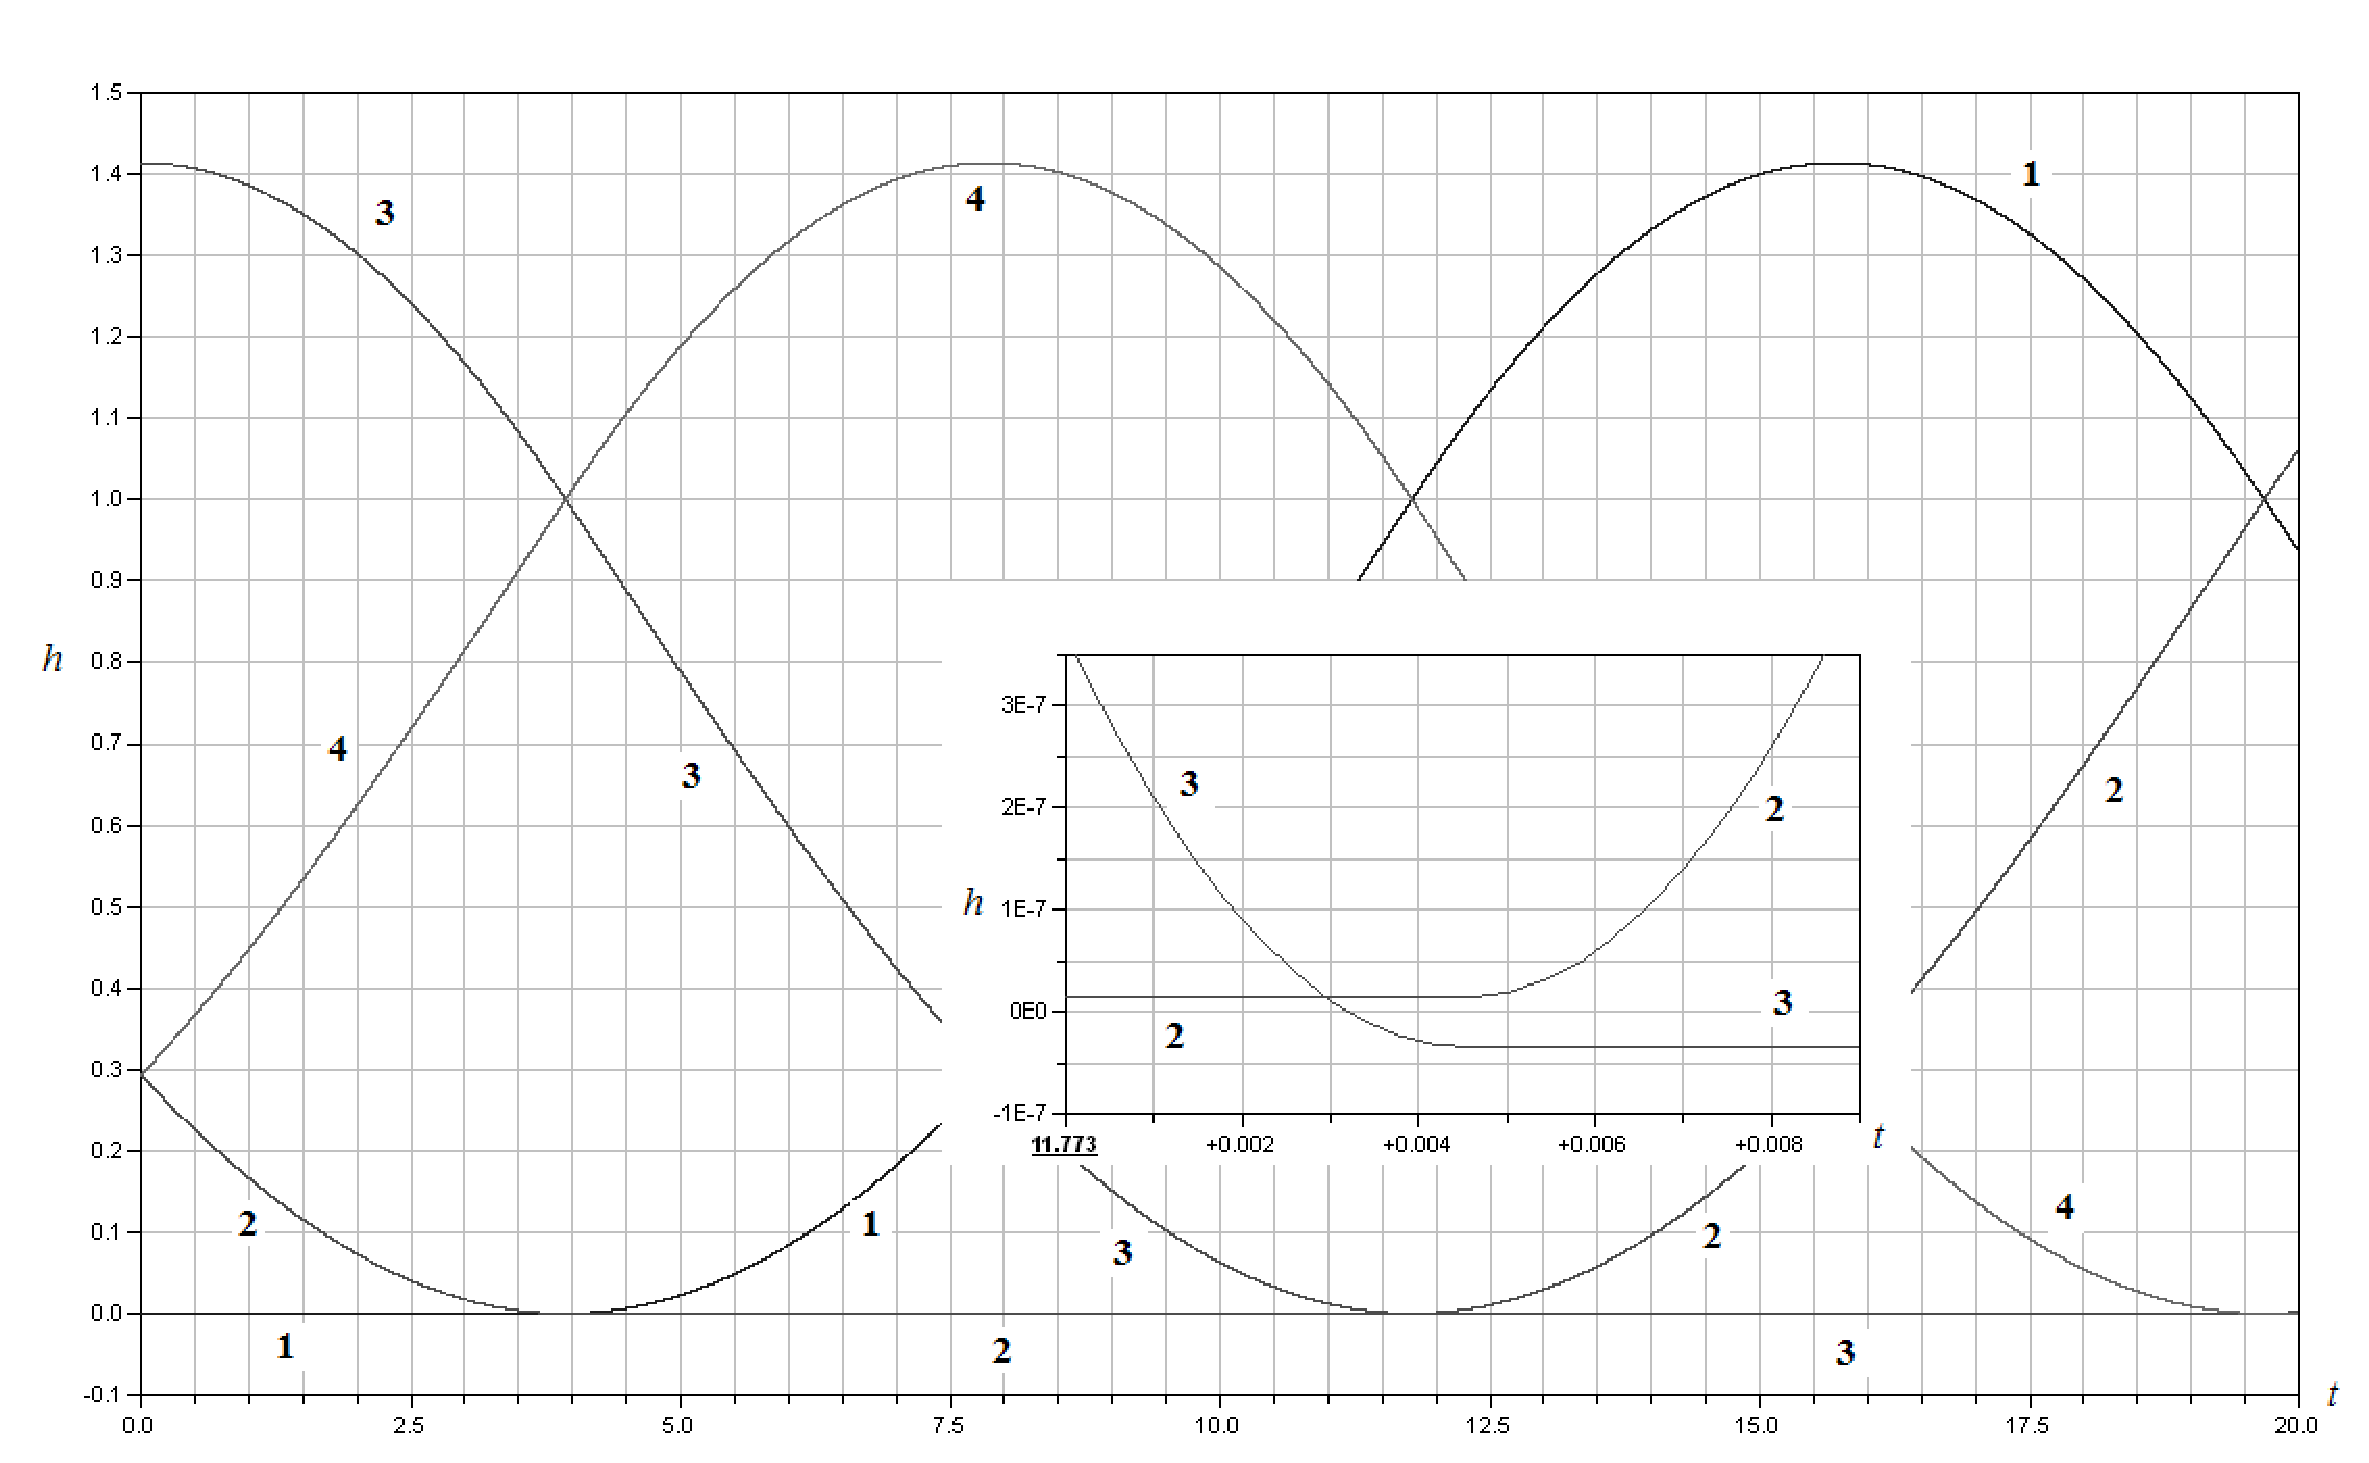
\includegraphics[width=15cm]{content/parts/3_friction/nd/Figure11.eps}}
\caption{Процесс смены роликов в контакте в численной модели.}
\label{fig1}
\end{figure}

Одновременно можно наблюдать точность соблюдения неудерживающей связи (Рис.~\ref{fig2}). Здесь обнаруживается процесс постепенного увеличения вычислительной ошибки -- расстояние между контактирующими телами медленно, для каждого последующего ролика в контакте, увеличивается. В то же время, абсолютная величина ошибки остается пренебрежимо малой -- около $10^{-7}$ от единицы длины. 

\begin{figure}[htb]
\centerline{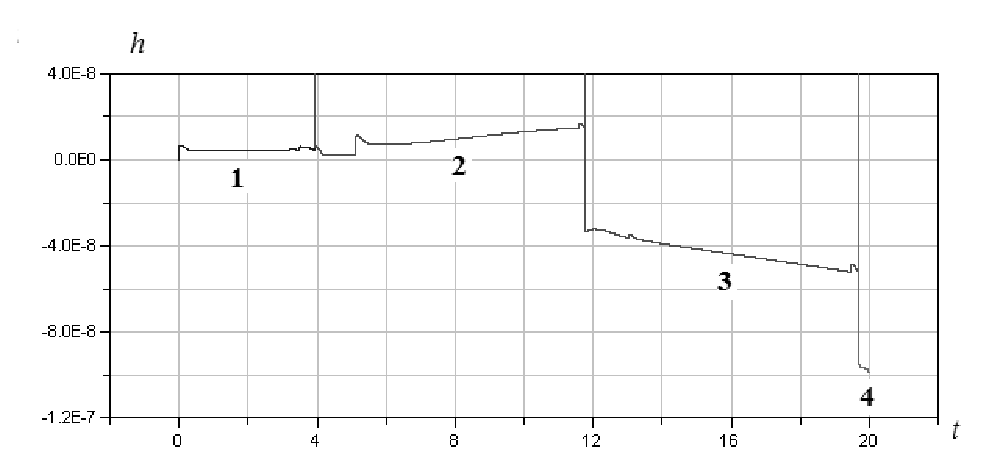
\includegraphics[width=15cm]{content/parts/3_friction/nd/Figure21.eps}}
\caption{Точность сохранения неудерживающей связи.}
\label{fig2}
\end{figure}

\subsection{Качественное сравнение модели с вязким трением и безынерционной модели}

Для модели с вязким трением были проведены расчеты, аналогичные движению 3 из главы 2. Конфигурация экипажа также симметрична, ролики усечены, на каждом колесе пять роликов.

Обнаружены динамические эффекты, аналогичные показанным в главе 2: характерный спиральный вид траектории центра масс на опорной плоскости возникает и в данной модели; видно раскручивание роликов; возрастание угловой скорости платформы экипажа, одновременное с убыванием поступательной скорости её центра; последующее медленное убывание угловой скорости; убывание кинетической энергии экипажа.

В данном расчете коэффициент вязкого трения принимался достаточно большим: $10^{5}$. Такое значение позволило моделировать ударный характер переходных процессов при смене ролика в контакте. На гладких участках движения сходство с движением неголономной модели соответствует результату \cite{karapetyan1981negolonom}.

\begin{figure}[htb]
\centerline{\includegraphics[width=\linewidth]{content/pic/new/visc_3_100.png}}
\caption{Характер движения системы с вязким трением при комбинации начальных условий движений 1 и 2. По оси абсцисс всюду, кроме правого верхнего графика отложено время}
\label{fig2}
\end{figure}



\chapter*{Выводы}

\begin{enumerate}

\item
Получены уравнения движения экипажа на омни-колесах по абсолютно шероховатой плоскости с учетом инерции роликов.

\item
Изучены свойства этих уравнений движения и проведено сравнение их с уравнениями движения безынерционной модели~\cite{Zobova2011}.

\item
Построен способ расчета изменения обобщенных скоростей при смене ролика в контакте, в предположении о мгновенном выполнении условия отсутствия проскальзывания между роликом и опорной плоскостью.

\item
Получены численные решения для симметричной конфигурации экипажа с омни-колесами с учетом ударного взаимодействия роликов и опорной плоскости.

\item
Построена динамическая модель экипажа с омни-колесами на плоскости с регуляризованным сухим трением. Показана возможность гладкого безударного переключения роликов в контакте в процессе качения/скольжения омни-колеса.

\item
Выполнена верификация динамической модели омни-экипажа с использованием безынерционной модели, рассмотренной в работе~\cite{Borisov2011}, в качестве предельного случая (когда суммарная масса роликов равна нулю).

\end{enumerate}



\newpage


\bibliographystyle{./util/BibTeX-Styles/utf8gost705u}  %% стилевой файл для оформления по ГОСТу

% \bibliography{content/omni}   % name your BibTeX data base

\addcontentsline{toc}{chapter}{Литература}
\bibliography{content/library}   % name your BibTeX data base


